%&"main"
% Fakesection 检错
% Fakesubsubsection 宏包
\RequirePackage[l2tabu, orthodox]{nag}
% Fakesubsubsection 编译器
\RequirePackage{ifxetex}
\RequireXeTeX

\documentclass{report}
% Fakesection 基础
% Fakesubsection 文字
% Fakesubsubsection 颜色
\usepackage{xcolor}
% Fakesubsubsection 长度
\usepackage{printlen}
\uselengthunit{mm}
% Fakesubsubsection 效果
\usepackage{ulem}
% Fakesubsubsection 字体
\usepackage{fontspec}
\setmainfont{Times New Roman}
% Fakesubsubsection 字体美化
\usepackage{microtype}
% Fakesubsubsection 字符边框
\usepackage{varwidth}
% Fakesubsection 断行
\usepackage{fvextra}
% Fakesubsubsection 标点
% XXX: load csquotes after fvextra to avoid warning <04-10-19> %
\usepackage{csquotes}
% Fakesubsection 样式
% Fakesubsubsection 目录
\usepackage{titletoc}
\titlecontents{chapter}[0pt]{\filright}{\contentspush{\thecontentslabel}}{}{\titlerule*{.}\contentspage}
% Fakesubsubsection 章节
\usepackage[
UTF8,
fontset = windows,
heading = true,
zihao = -4,
sub4section,
]{ctex}
\setCJKfamilyfont{zhsong}[AutoFakesubBold = {2.17}]{SimSun}
\renewcommand*{\songti}{\CJKfamily{zhsong}}
\ctexset{
	chapter = {
		name = 实验,
		aftername = \hspace{1\ccwd},
		format = \centering\zihao{3}\heiti\bfseries,
		beforeskip = 0.5\ccwd,
		afterskip = 0.5\ccwd,
	},
	section = {
		name = ,
		number = \chinese{section},
		aftername = 、,
		format = \zihao{-3}\heiti\bfseries,
		beforeskip = 0.5\ccwd,
		afterskip = 0.5\ccwd,
	},
	subsection = {
		format = \zihao{4}\heiti\bfseries,
	}
}
% Fakesubsubsection 图表
\usepackage{caption}
\captionsetup[figure]{labelsep=space}
\captionsetup[table]{labelsep=space}
\captionsetup{font=small}
\setlength{\abovecaptionskip}{0.5\ccwd}
\setlength{\belowcaptionskip}{0.5\ccwd}
% Fakesubsubsection 子图表
\usepackage{subcaption}
% Fakesubsubsection 公式
\setlength{\abovedisplayskip}{0.5em}
\setlength{\belowdisplayskip}{0.5em}
% Fakesubsubsection 列表
\usepackage{enumitem}
\setlist[enumerate, 1]{
	fullwidth,
	label = (\arabic*),
	font = \textup,
	itemindent=2em
}
\setlist[enumerate, 2]{
	fullwidth,
	label = (\alph*),
	font = \textup,
	itemindent=4em
}
% Fakesubsubsection 代码
% XXX: need -shell-escape & pygmentize <04-10-19> %
\usepackage{minted}
\usepackage{boxie}
% XXX: avoid boxie's warning <04-10-19> %
\makeatletter
\xdefinecolor{tcbcol@back}{rgb}{0,0,0}
\makeatother
% Fakesubsubsection 问答
\usepackage{exercise}
\usepackage{tasks}
% Fakesubsubsection 改动

% Fakesection 插入
% Fakesubsection 表格
% Fakesubsubsection 三线
\usepackage{booktabs}
% Fakesubsubsection 对角线
\usepackage{diagbox}
% Fakesubsubsection 合并列
\usepackage{multicol}
% Fakesubsubsection 合并行
\usepackage{multirow}
% Fakesubsubsection 分割单元格
\usepackage{makecell}
% Fakesubsubsection 短表
\usepackage{tabu}
% Fakesubsubsection 长表
\usepackage{longtable}
% Fakesubsubsection 彩色表
\usepackage{fancybox}
\usepackage{colortbl}
\usepackage{tcolorbox}
\tcbuselibrary{skins}
\tcbuselibrary{breakable}
\tcbuselibrary{theorems}
\tcbuselibrary{listings}
\tcbuselibrary{xparse}
% XXX: need -shell-escape & pygmentize <04-10-19> %
\tcbuselibrary{minted}
% Fakesubsubsection 导入数据
\usepackage{csvsimple}
% Fakesubsection 图形
% Fakesubsubsection 插图
\usepackage{graphicx}
\graphicspath{{fig/}{etc/}}
% Fakesubsubsection 环绕
\usepackage{wrapfig}
% Fakesubsubsection 图片重叠
\usepackage{overpic}
% Fakesubsubsection 徽标
\usepackage{hologo}
% Fakesubsubsection 条形码
\usepackage{ean13isbn}
% Fakesubsubsection 二维码
\usepackage{qrcode}
% Fakesubsection 符号
% Fakesubsubsection 数学符号
\usepackage{amsfonts}
\usepackage{amsmath}
\usepackage{latexsym}
\usepackage{textcomp}
\usepackage{bm}
% Fakesubsubsection 幻灯片符号
\usepackage{pifont}
% Fakesubsubsection 大数学符号
\usepackage{exscale}
% Fakesubsubsection 数学符号放缩
\usepackage{relsize}
% Fakesubsubsection 公式
\usepackage{cases}
\usepackage{physics}
% Fakesubsubsection 单位
\usepackage{siunitx}
% Fakesubsubsection 计算机
% Fakesubsection 媒体
\usepackage{media9}
% Fakesubsection 链接
\usepackage[
colorlinks = true,
linkcolor = gray,
citecolor = gray,
backref = page
]{hyperref}
% Fakesubsection 批注
\usepackage{todonotes}
\usepackage{cooltooltips}
\usepackage{pdfcomment}
% Fakesubsection 文本框
\usepackage{boxedminipage2e}
% Fakesubsection 页眉页脚
\usepackage{fancyhdr}
\fancypagestyle{plain}{
	\pagestyle{fancy}
}

% Fakesection 设计
% Fakesubsection 水印
\usepackage{wallpaper}
% Fakesubsection 主题

% Fakesection 布局
% Fakesubsection 页面
\usepackage{geometry}
% Fakesubsection 缩进
\usepackage{indentfirst}
% Fakesubsection 间距
\usepackage{setspace}
\usepackage[
restoremathleading=false,
UseMSWordMultipleLineSpacing,
MSWordLineSpacingMultiple=1.5
]{zhlineskip}
% Fakesection 引用
% Fakesubsection 脚注
\renewcommand{\thefootnote}{\fnsymbol{footnote}}
\renewcommand{\thempfootnote}{\fnsymbol{mpfootnote}}
% Fakesubsection 引文
\usepackage{morewrites}
\usepackage[square, comma, numbers, super, sort&compress, longnamesfirst, sectionbib, nonamebreak]{natbib}
% Fakesubsection 题注
\usepackage{epigraph}
% Fakesubsection 索引
\usepackage{makeidx}
\makeindex
% Fakesubsection 关联
% XXX: need amsmath <04-10-19> %
\numberwithin{Exercise}{chapter}
\numberwithin{Answer}{chapter}

% Fakesection 特殊功能
% Fakesubsection 页数统计
\usepackage{lastpage}
% Fakesubsection 数学表达式
\usepackage{calc}

\begin{document}
% Fakesection 扉页

\begin{titlepage}
	\centering

	\begin{spacing}{1.5}
		\zihao{4}
		\vfill
	\end{spacing}

	\begin{spacing}{1.5}
		\fontsize{30pt}{30pt}\selectfont\kaishu
		\vspace{0.5em}

		南~京~理~工~大~学

		\vspace{0.2em}
	\end{spacing}

	\begin{spacing}{1.5}
		\fontsize{45pt}{45pt}\selectfont
		\textbf{EDA设计(I)}

		\textbf{实验报告}
	\end{spacing}

	\begin{spacing}{1}
		\zihao{-1}
		\vspace{3em}
	\end{spacing}

	\begin{spacing}{2}
		\fontsize{16pt}{16pt}\selectfont
		\begin{tabu}to.8\linewidth{@{}X[5,r]@{}X[c]@{}X[6,l]@{}X[5,r]@{}X[c]@{}X[6,l]@{}}
			\makebox[4\ccwd][s]{\bf 作者}      & :&\underline{\makebox[6\ccwd][c]{\kaishu 吴振宇}} & \makebox[4\ccwd][s]{\bf 学号}      & :&\underline{\makebox[6\ccwd][c]{916101630117}}\\
			\makebox[4\ccwd][s]{\bf 学院(系)}      & :&\multicolumn{4}{c}{\underline{\makebox[16\ccwd][c]{\kaishu 电子工程与光电技术学院}}}\\
			\makebox[4\ccwd][s]{\bf 专业}      & :&\multicolumn{4}{c}{\underline{\makebox[16\ccwd][c]{\kaishu 电子信息工程}}}
		\end{tabu}

		\vspace{1em}

		\begin{tabu}to.6\linewidth{@{}X[4,r]@{}X[c]@{}X[12,l]@{}}
			\makebox[4\ccwd][s]{\bf 指导老师}  & :&\underline{\makebox[12\ccwd][c]{\kaishu 吴少琴}}\\
			\makebox[4\ccwd][s]{\bf 实验日期}  & :&\underline{\makebox[12\ccwd][c]{\kaishu\number\year 年9月14日}}
		\end{tabu}

		\vspace{1em}
	\end{spacing}

	\begin{spacing}{2}
		\fontsize{18pt}{18pt}\selectfont\heiti
		\number\year 年9月
	\end{spacing}

\end{titlepage}

% Fakesection 摘要

\renewcommand{\abstractname}{\zihao{3}\heiti\textbf{摘\hspace{2\ccwd}要}}
\begin{abstract}
	\vspace{1\ccwd}

	本文根据题目条件,正确设计了满足要求的放大电路,并对其进行了指标的计算、计算机仿真,在最后根据计算结果对仿真结果进行误差分析。\cite{1989模拟电子技术基础,2004模拟电子技术基础简明教程,吴少琴2009电子元器件在电路仿真中的建模}

	实验一,成功设计了合理的单级放大电路,测量了三极管的参数以及放大电路的参数。

	实验二,在单级放大电路的基础上设计了差分放大电路,测量了共模增益和差模增益,\textbf{验证了差分放大能抑制共模信号的结论}。

	实验三,在单级放大电路的基础上设计了两级放大电路,并设计了反馈电阻,测量了开环和闭环两种情况下的放大参数,\textbf{验证了闭环能稳定放大参数的结论}。

	实验四,设计了阶梯波发生器,能通过调节元器件参数改变阶梯波波形。并\textbf{设计了符合要求的只用三极管的阶梯波发生器和反向阶梯波发生器}。

	\vspace{2\ccwd}

	\noindent\textbf{关键词}\hspace{1\ccwd}放大电路\hspace{1\ccwd}计算机仿真\hspace{1\ccwd}阶梯波发生器
\end{abstract}

\renewcommand{\abstractname}{\zihao{3}\textbf{Abstract}}
\begin{abstract}
	\vspace{1em}

	According to the condition of the subject, this paper correctly designs the amplifier circuit which meets the requirement, calculates its index, simulates it by computer, and finally analyses the error of the simulation result according to the calculation result.

	In experiment 1, a reasonable single-stage amplifier circuit was successfully designed, and the parameters of transistor and amplifier circuit were measured.

	In experiment 2, a differential amplifier circuit is designed based on the single-stage amplifier circuit. The common-mode gain and differential-mode gain are measured, and \textbf{the conclusion that differential amplification can suppress common-mode signal is verified}.

	In experiment 3, a two-stage amplifier circuit is designed on the basis of a single-stage amplifier circuit, and a feedback resistor is designed to measure the amplification parameters in both open-loop and closed-loop cases, which \textbf{verifies the conclusion that the closed-loop can stabilize the amplification parameters}.

	In experiment 4, a step wave generator is designed, which can change the parameters of step wave by adjusting the parameters of components. \textbf{A step-wave generator and a reverse step-wave generator using only transistors are designed to meet the requirements}.

	\vspace{2em}

	\noindent\textbf{Keywords}\hspace{1em}Amplifier Circuit\hspace{1em}Computer Simulation\hspace{1em}Stepped Wave Generator
\end{abstract}

% Fakesection 单面目录页眉页脚

\pagestyle{fancy}
\renewcommand{\headrulewidth}{0pt}
\lhead{}
\chead{\small{\leftmark}}
\rhead{\small{第\thepage 页}}
\lfoot{}
\cfoot{}
\rfoot{}

% Fakesection 目录

\pagenumbering{roman}

\tableofcontents
\listoffigures
\listoftables

\newpage

\renewcommand{\ExerciseName}{问题}
\renewcommand{\AnswerName}{回答}
% XXX: make listexercisename center <04-10-19> %
\renewcommand{\listexercisename}{}
\chead{问题}

\begin{center}
	\zihao{3}\heiti
	\mbox{}

	问题
	\vspace{-1\ccwd}
\end{center}

\listofexercises

\newpage
\chead{\small{\leftmark}}
\pagenumbering{arabic}

% Fakesection 单面正文页眉页脚

\lhead{\small{\rightmark}}
\rhead{\small{第\thepage 页~共~\pageref{LastPage}~页}}

% Fakesection 正文

\chapter{单级放大电路的设计与仿真}%
\label{cha:单级放大电路的设计与仿真}

\section{实验目的}%
\label{sec:\arabic{chapter}实验目的}

\begin{enumerate}
	\item 设计一个分压偏置的单管电压放大电路,要求电压增益大于50,输出电阻设计在\SI{5}{\kohm}以内,带宽大于\SI{500}{\kHz}。
	\item 已知供电电源为\SI{12}{\V},三极管型号BC817-16,负载电阻为\SI{20}{\kohm}。输入信号为:频率为\SI{10}{\kHz},峰值\SI{1}{\mV}$ \sim $\SI{5}{\mV}的正弦信号。
	\item 放大器指标测量:在放大器输入端接入正弦信号,调节电路静态工作点(调节偏置电阻),观测电路输出信号,使得输出波形不失真。在此状态下测试:

		\begin{enumerate}
			\item 电路静态工作点值;
			\item 三极管的输入、输出特性曲线和$ \beta $、$ r_\mathrm{be} $、$ r_\mathrm{ce} $值 ;
			\item 利用示波器得到输出波形,求出该放大电路的放大倍数;
			\item 利用交流扫描分析(ACAnalysis/ACSweep)画出电路电压增益的幅频特性和相频特性;
			\item 利用交流扫描分析画出输出变量为$ R_\mathrm{i} = \dfrac{V_\mathrm{i}}{I_\mathrm{i}} $的频率特性曲线图,读出电路工作频率\SI{10}{\kHz}时的值,从而得到电路输入电阻的值;
			\item 将信号源$ V_\mathrm{i} $短路,负载电阻用一个信号源$ V_\mathrm{T} $替代。再进行交流扫描分析,画出输出变量$ R_\mathrm{o} = \dfrac{V_\mathrm{T}}{I_\mathrm{T}} $,读出电路对应工作频率下的值,从而得到电路输出电阻的值。
		\end{enumerate}

	\item 观察失真波形:调节电路静态工作点(调节偏置电阻),观察电路出现饱和失真和截止失真的输出信号波形,并测试对应的静态工作点值。
\end{enumerate}

\section{实验要求}%
\label{sec:\arabic{chapter}实验要求}

\begin{Exercise}
	给出单级放大电路原理图。
\end{Exercise}

\begin{Answer}
	单级放大电路原理图见图\ref{fig:单级放大电路原理图}。
\end{Answer}

\begin{Exercise}
	电路工作在不失真状态下:

	\begin{enumerate}
		\item 给出三极管静态工作点的测量值;
		\item 给出测试三极管在该工作点下的值$ \beta $、$ r_\mathrm{be} $、$ r_\mathrm{ce} $的实验图和测试结果;
		\item 给出输出波形图,求出放大倍数,并与理论计算值进行比较;
		\item 给出电路的幅频和相频特性图,并得出下限截止频率$ f_\mathrm{L} $、上限截止频率$ f_\mathrm{H} $以及带宽BW值;
		\item 给出输入电阻的幅频特性图,求出工作频率下输入电阻的测试结果,并和理论计算值进行比较;
		\item 给出测量输出电阻的实验图,以及输出电阻的幅频特性图,求出工作频率下输出电阻的测试结果,并和理论计算值进行比较。
	\end{enumerate}

\end{Exercise}

\begin{Answer}
	单级放大电路失真参数见表\ref{tab:单级放大电路失真指标},三极管参数见表\ref{tab:三极管参数},频率响应见图\ref{fig:单级放大电路增益},输入电阻和输出电阻见章节\ref{sub:\arabic{chapter}误差分析}。
\end{Answer}

\begin{Exercise}
	给出电路饱和失真和截止失真时输出电压的波形图。并给出两种状态下三极管的静态工作点值。分析出现失真原因。
\end{Exercise}

\begin{Answer}
	饱和失真波形图见图\ref{fig:单级放大电路饱和失真},截止失真波形图见图\ref{fig:单级放大电路截止失真}。静态工作点见表\ref{tab:单级放大电路参数},失真原因见章节\ref{sub:\arabic{chapter}仿真结果}。
\end{Answer}

\section{实验步骤}%
\label{sec:\arabic{chapter}实验步骤}

\subsection{设计电路}%
\label{sub:\arabic{chapter}设计电路}

\begin{figure}[H]
	\centering
	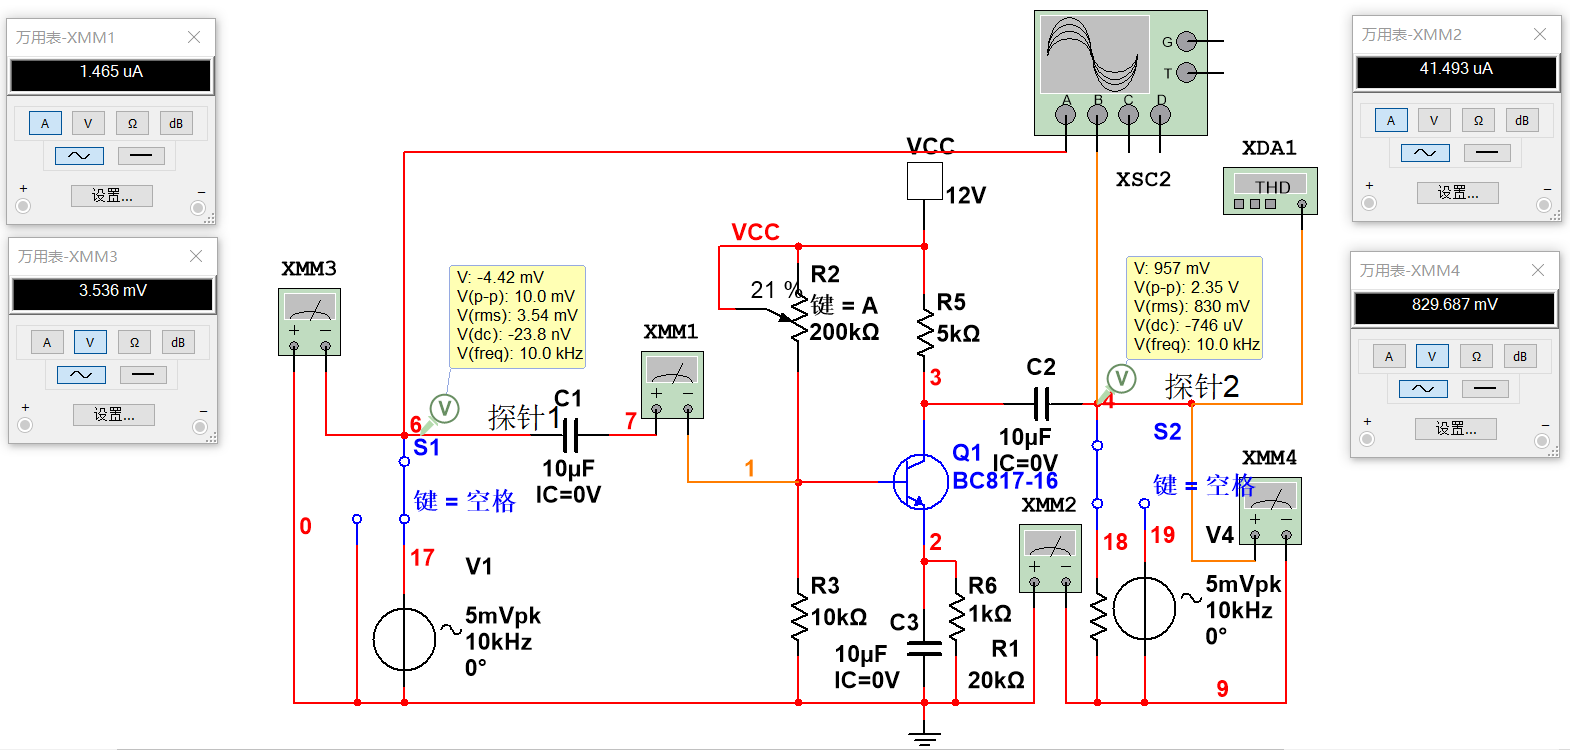
\includegraphics[width=0.8\linewidth]{1/Ri.png}
	\caption{单级放大电路原理图}
	\label{fig:单级放大电路原理图}
\end{figure}

单级放大电路原理图如图\ref{fig:单级放大电路原理图}所示,采用分压式偏置电路,有效稳定静态工作点。

其中$ R_3, R_2 $为偏置电阻,$ V_\mathrm{be} = \dfrac{R_2}{R_2 + R_3} V_\mathrm{cc} $,通过调节$ R_2 $阻值大小可以改变$ V_\mathrm{be} $进而改变静态工作点;

$ R_6 $具有直流负反馈作用,帮助稳定静态工作点,而$ C_3 $则是在交流通路中将$ R_6 $短路,增大电路放大倍数;

$ C_1, C_2 $都是耦合电容,隔直通交,其中$ C_1 $是避免交流小信号影响静态工作点,C2是滤除直流信号,避免静态工作点影响输出信号。

\subsection{指标计算}%
\label{sub:\arabic{chapter}指标计算}

\begin{figure}[H]
	\centering
	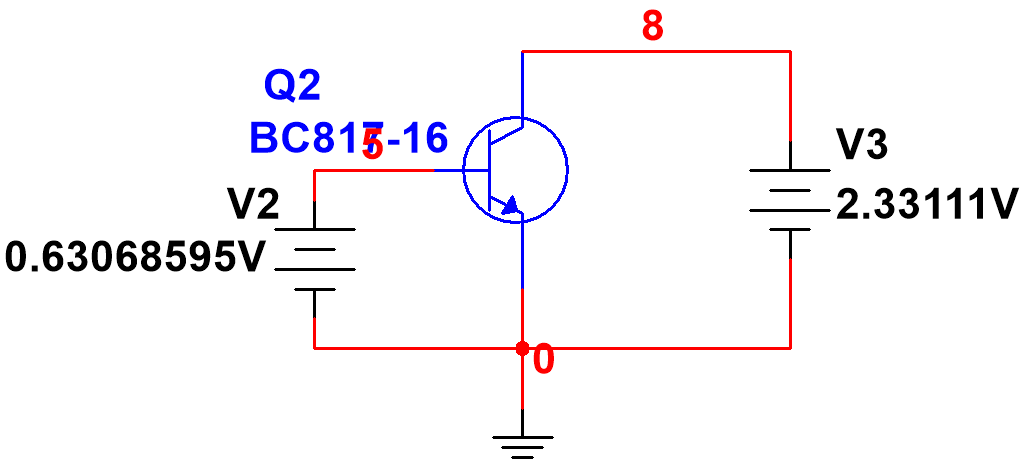
\includegraphics[width=0.8\linewidth]{1/measure.png}
	\caption{测量}
	\label{fig:测量}
\end{figure}

\begin{figure}[H]
	\centering
	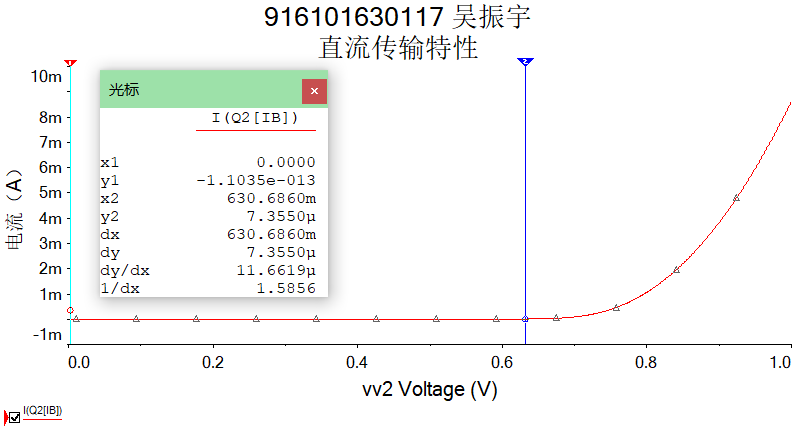
\includegraphics[width=0.8\linewidth]{1/input.png}
	\caption{输入特性曲线}
	\label{fig:输入特性曲线}
\end{figure}

\begin{figure}[H]
	\centering
	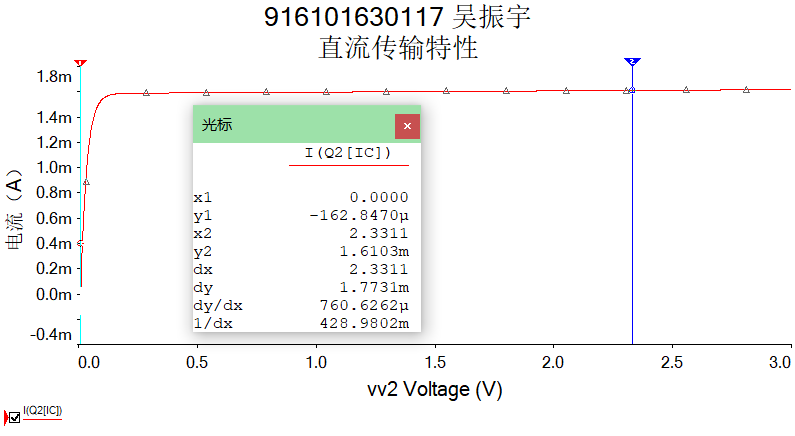
\includegraphics[width=0.8\linewidth]{1/output.png}
	\caption{输出特性曲线}
	\label{fig:输出特性曲线}
\end{figure}

根据要求,输出电阻决定了图\ref{fig:单级放大电路原理图}中$ R_5 $为\SI{5}{\kohm}。其它参数选取适当。

\subsection{仿真结果}%
\label{sub:\arabic{chapter}仿真结果}

\begin{table}[H]
	\centering
	\caption{单级放大电路失真指标}
	\label{tab:单级放大电路失真指标}
	\csvautobooktabular{tab/1/1-1.csv}
\end{table}

\begin{table}[H]
	\centering
	\caption{三极管参数}
	\label{tab:三极管参数}
	\csvautobooktabular{tab/1/1-2.csv}
\end{table}

\begin{table}[H]
	\centering
	\caption{单级放大电路参数}
	\label{tab:单级放大电路参数}
	\csvautobooktabular{tab/1/1-3.csv}
\end{table}

\subsubsection{饱和失真}%
\label{ssub:饱和失真}

饱和失真主要是将静态工作点调整至饱和区附近。

\begin{figure}[H]
	\centering
	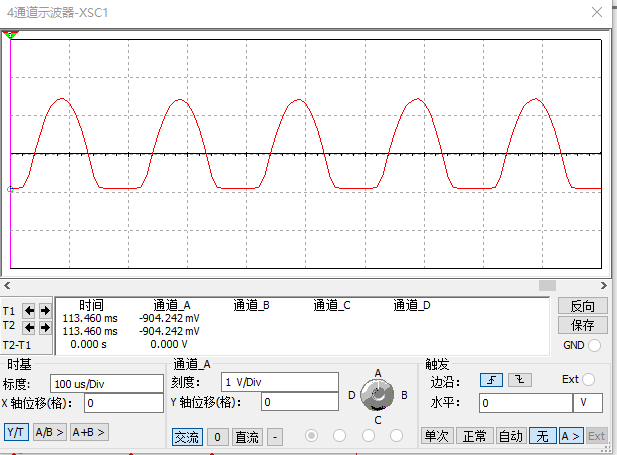
\includegraphics[width=0.8\linewidth]{1/saturation.png}
	\caption{单级放大电路饱和失真}
	\label{fig:单级放大电路饱和失真}
\end{figure}

饱和失真波形如图\ref{fig:单级放大电路饱和失真}所示,由于是反相放大器,所以饱和失真削弱了下半周期,出现削平波形。

\subsubsection{截止失真}%
\label{ssub:截止失真}

截止失真主要是将静态工作点调整至截止区附近,同时注意不能太靠近截止区,否则放大倍数受影响,失真波形不明显。

\begin{figure}[H]
	\centering
	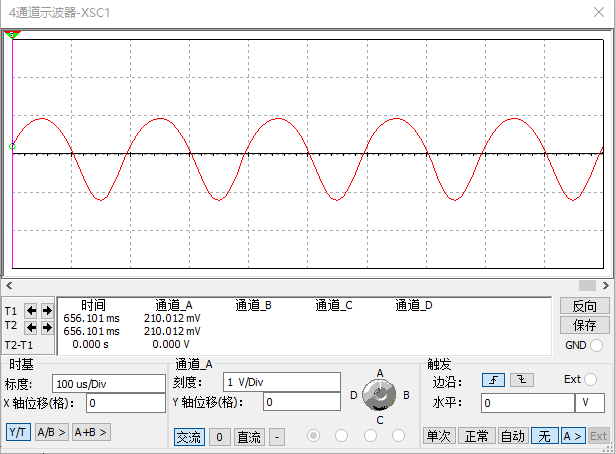
\includegraphics[width=0.8\linewidth]{1/cutoff.png}
	\caption{单级放大电路截止失真}
	\label{fig:单级放大电路截止失真}
\end{figure}

截止失真波形如图\ref{fig:单级放大电路截止失真}所示,由于是反相放大器,所以饱和失真削弱了上半周期,出现削平波形。

\subsubsection{最大不失真}%
\label{ssub:最大不失真}

最大不失真主要是将静态工作点调整至放大区中间,即能够实现最大不失真信号幅度的测量。

主要方法是先调节到恰好饱和失真、截止失真,测量静态工作点电压并取其平均值即为最大不饱和失真静态工作点附近;再通过细微调整确定最大不失真静态工作点以及输出幅值。

图\ref{fig:输出特性曲线}为BC817-16管输出特性曲线,通过比较交流负载线与输出特性曲线交点可知理论上最大不失真静态工作点$ V_\mathrm{ce} $约为\SI{3.7}{\V}左右,与实验所得结果\SI{3.95}{\V}吻合。

\begin{figure}[H]
	\centering
	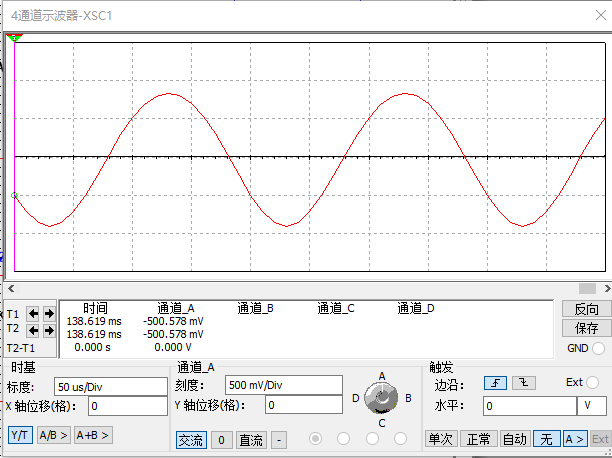
\includegraphics[width=0.8\linewidth]{1/normal.png}
	\caption{单级放大电路最大不失真}
	\label{fig:单级放大电路最大不失真}
\end{figure}

图\ref{fig:单级放大电路最大不失真}即最大不失真输出波形,其中输入电压峰值\SI{5}{\mV},输出电压峰值1.6V左右。上半周期波形峰值略小于下半周期波形,这是由于输出特性曲线靠近截止区时曲线略有上移引起的非线性失真,属于正常情况。

\subsubsection{单级放大电路输入电阻}%
\label{ssub:单级放大电路输入电阻}

如图\ref{fig:单级放大电路原理图}所示即为输入电阻测量电路,即断开输出电阻,输入端添加一个信号源。

\subsubsection{单级放大电路输出电阻}%
\label{ssub:单级放大电路输出电阻}

如图\ref{fig:单级放大电路输出电阻}所示即为输出电阻测量电路,即短路输入端电压源,输出端断开输出电阻,添加一个信号源。

\begin{figure}[H]
	\centering
	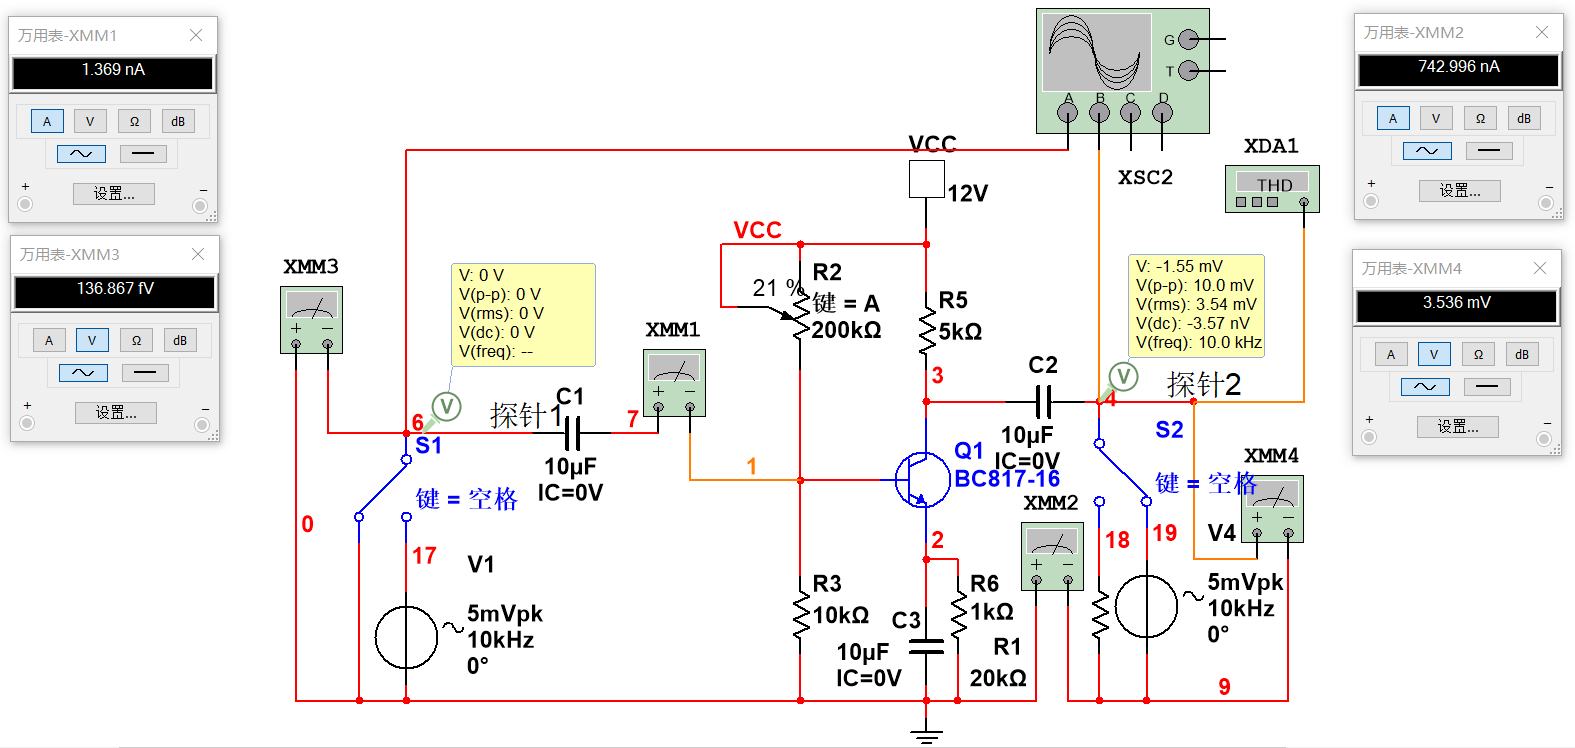
\includegraphics[width=0.8\linewidth]{1/Ro.png}
	\caption{单级放大电路输出电阻}
	\label{fig:单级放大电路输出电阻}
\end{figure}

\subsubsection{频率响应}%
\label{ssub:频率响应}

频率响应原理图如图\ref{fig:单级放大电路原理图}所示,其中信号源峰值\SI{5}{\mV},频率\SI{10}{\kHz}。

采用交流分析时添加公式$ V(3)/V(1) $即为放大倍数,注意单位选为\SI{}{\dB}。

如图\ref{fig:单级放大电路增益}中频增益为\SI{41.43}{\dB},中频增益减\SI{3}{\dB}即为上下限增益数值,对应即为上下界频率。

\begin{figure}[H]
	\centering
	\begin{subfigure}[H]{.8\linewidth}
		\centering
		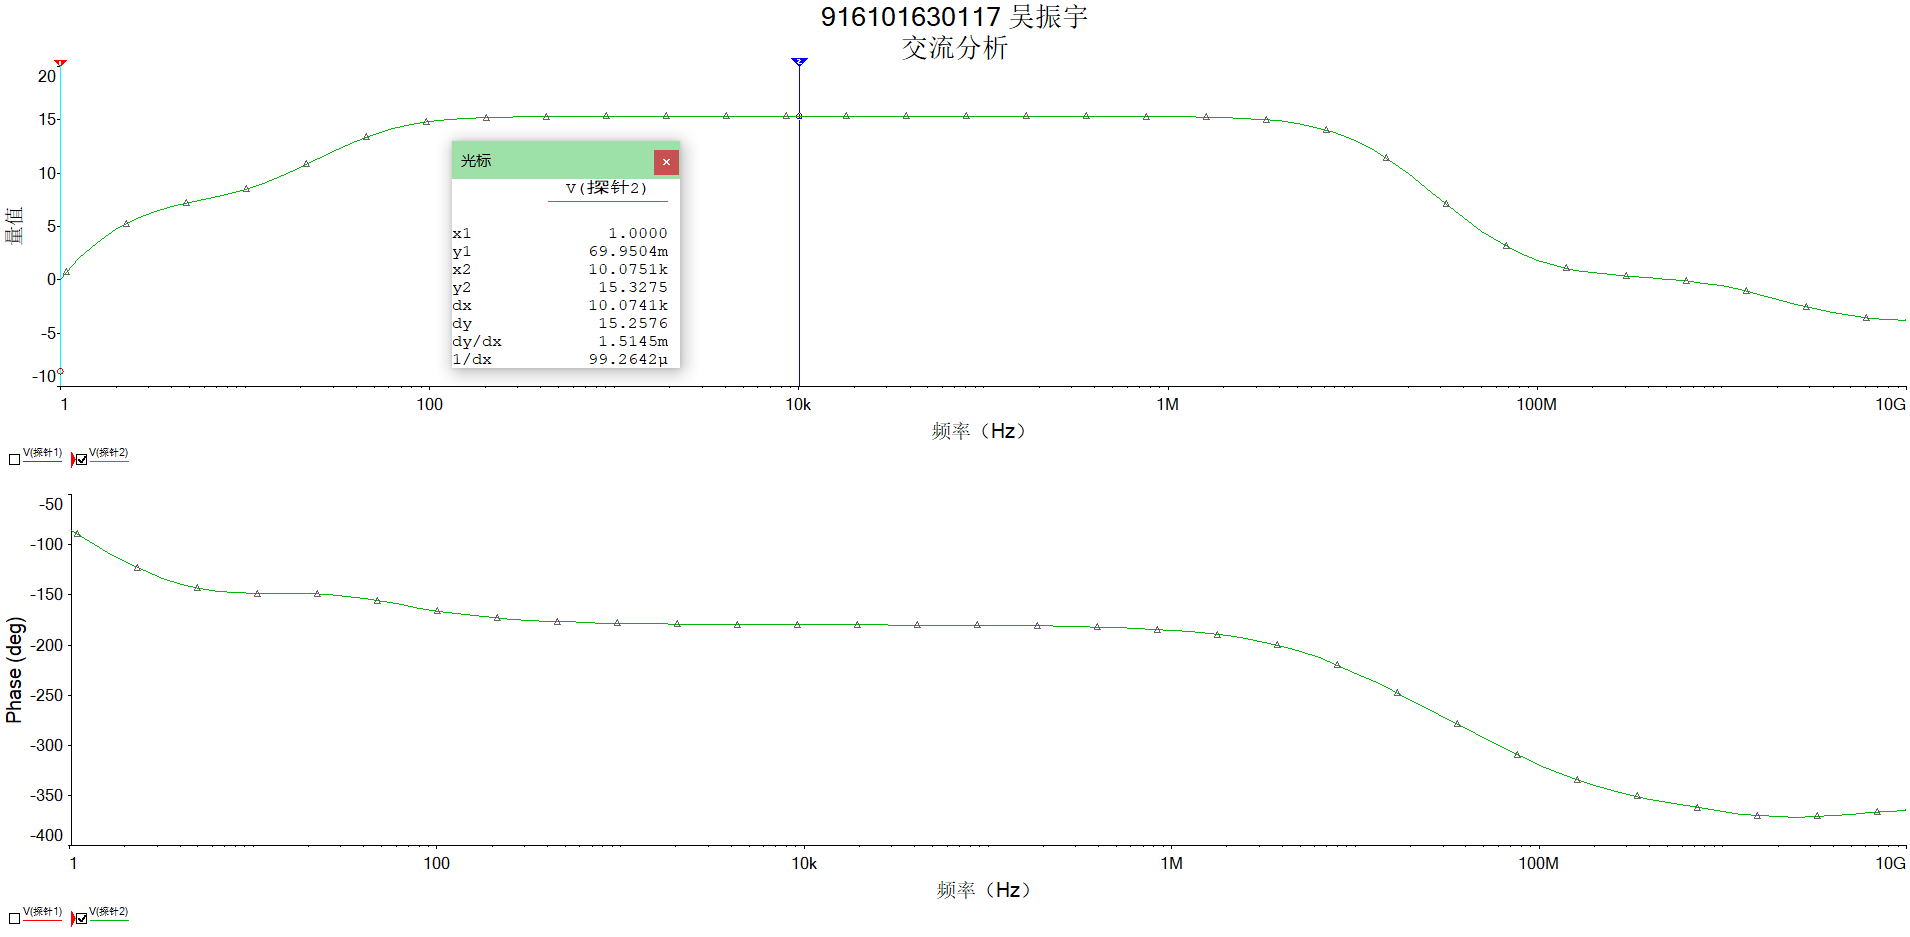
\includegraphics[width=\linewidth]{1/f.png}
		\caption{单级放大电路中频增益}
		\label{fig:单级放大电路中频增益}
	\end{subfigure}
	\quad
	\begin{subfigure}[H]{.8\linewidth}
		\centering
		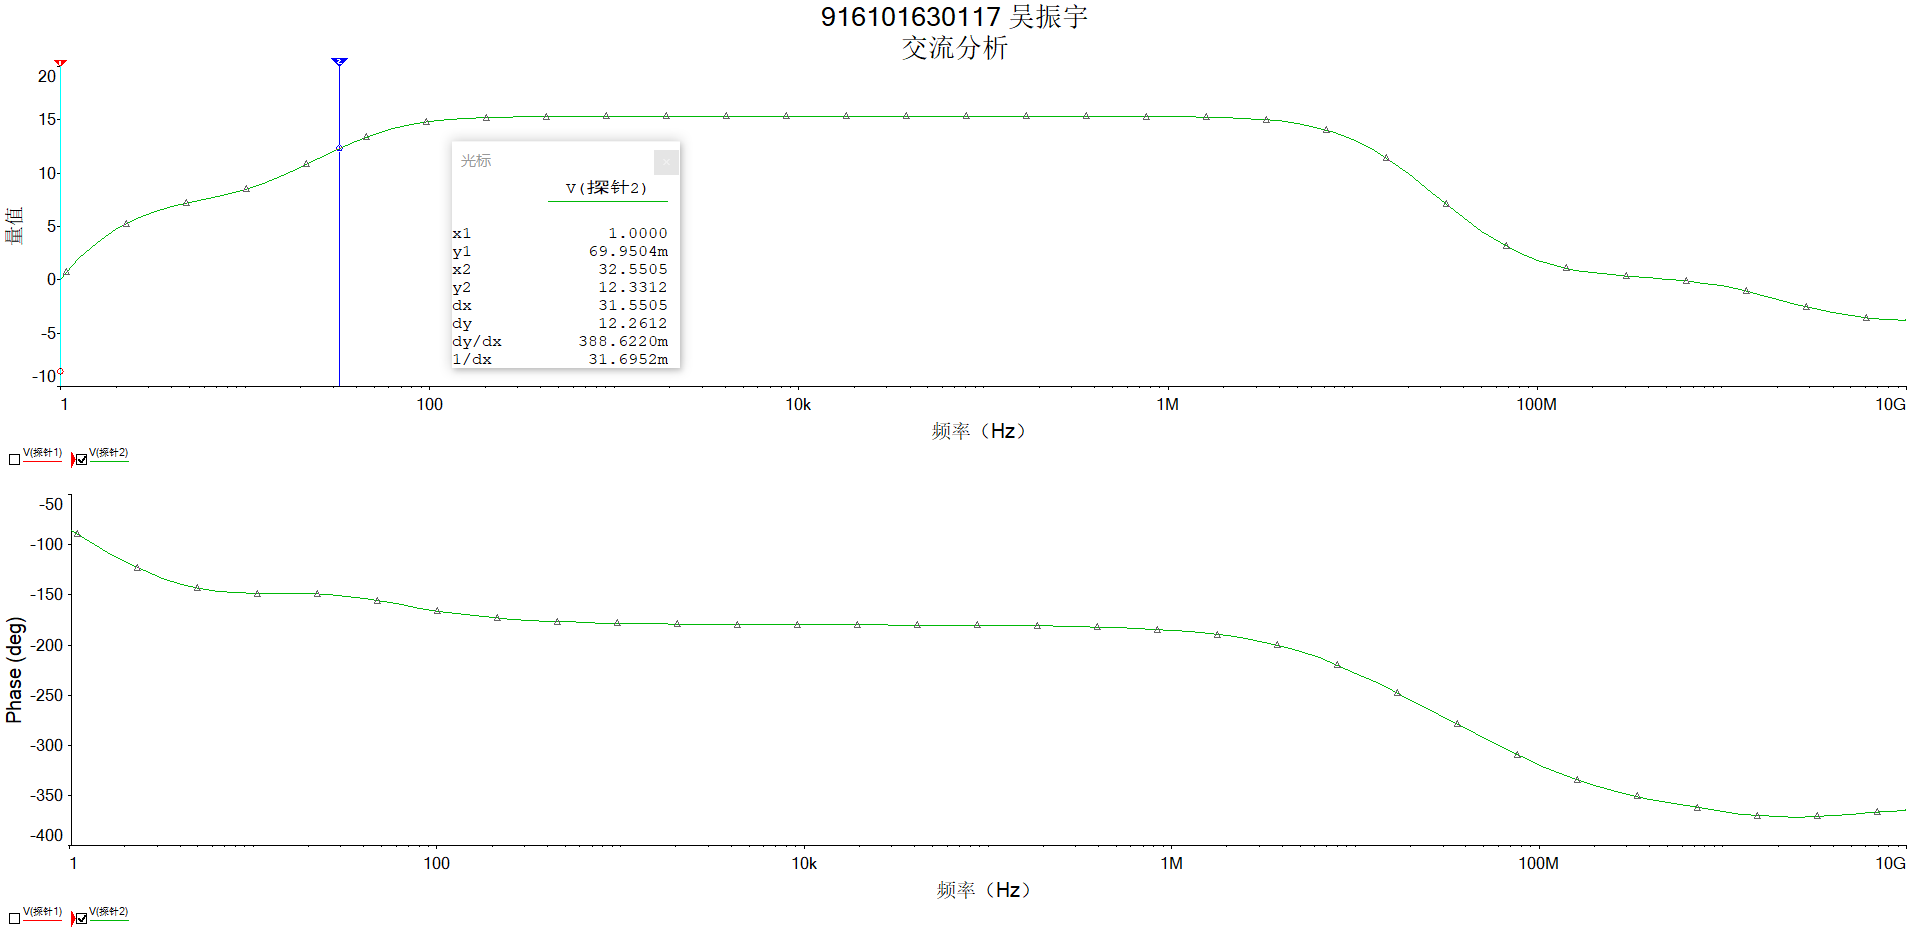
\includegraphics[width=\linewidth]{1/fL.png}
		\caption{单级放大电路下限增益}
		\label{fig:单级放大电路下限增益}
	\end{subfigure}
	\quad
	\begin{subfigure}[H]{.8\linewidth}
		\centering
		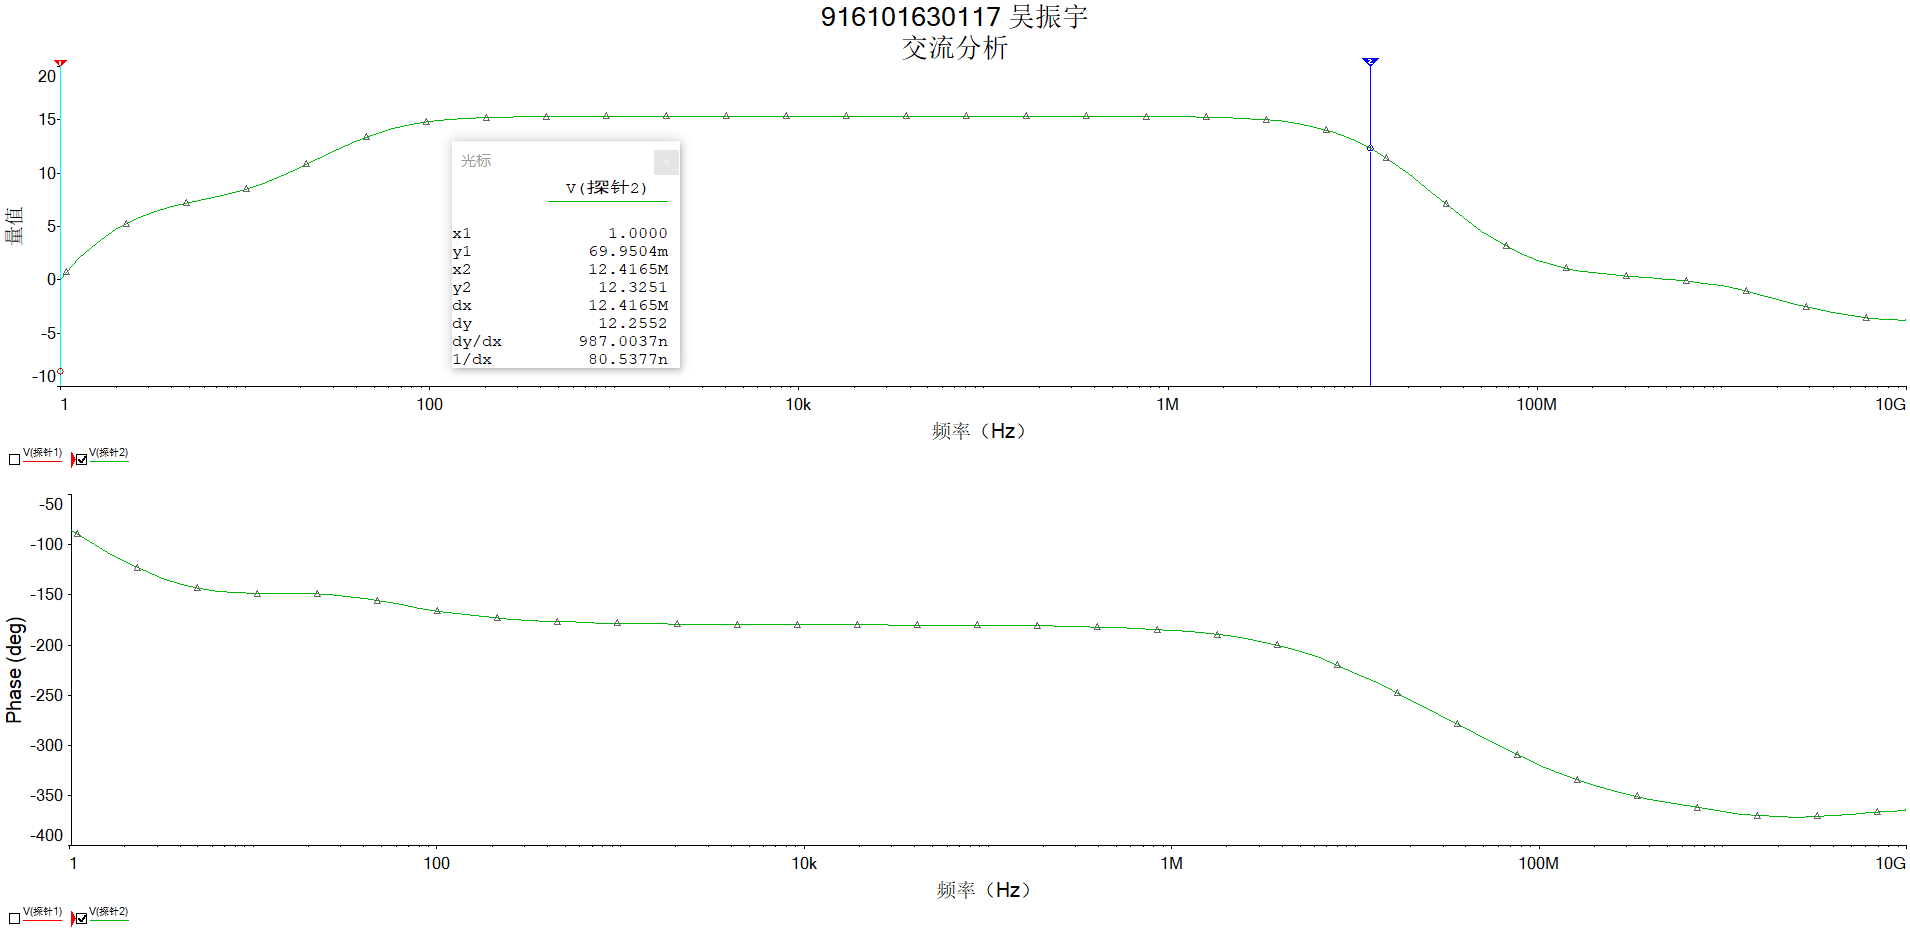
\includegraphics[width=\linewidth]{1/fH.png}
		\caption{单级放大电路上限增益}
		\label{fig:单级放大电路上限增益}
	\end{subfigure}
	\caption{单级放大电路增益}
	\label{fig:单级放大电路增益}
\end{figure}

\subsection{误差分析}%
\label{sub:\arabic{chapter}误差分析}

\subsubsection{输入电阻误差分析}%
\label{ssub:输入电阻误差分析}

采用交流分析法测量输入电阻,图\ref{fig:输入交流通路}为输入交流通路。由图可知输入电阻理论值为$ (R_2+R_3)\parallel R_5\parallel r_\mathrm{be} $

\begin{figure}[H]
	\centering
	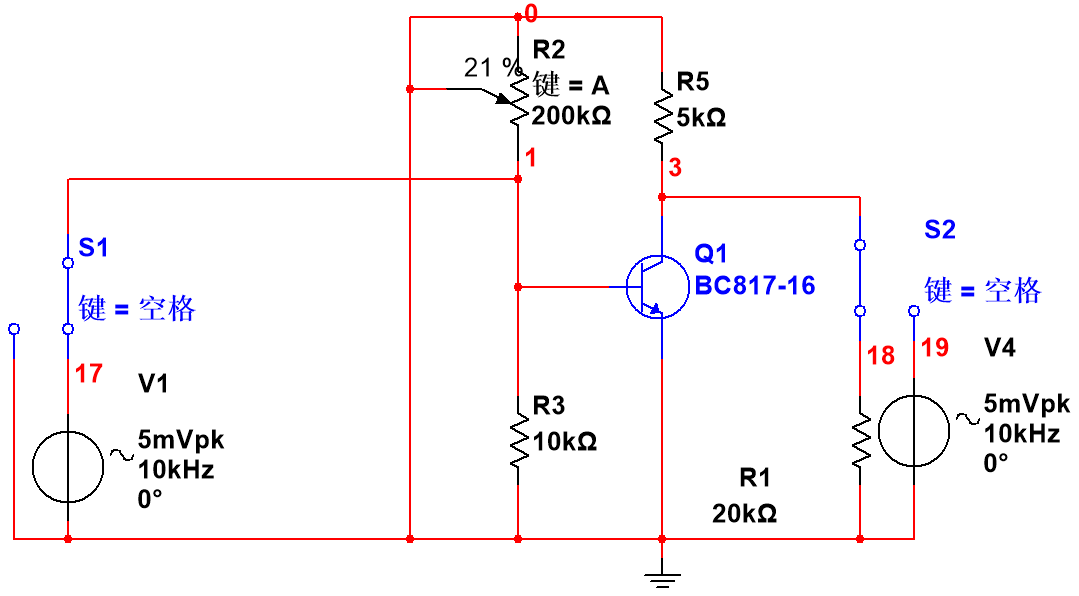
\includegraphics[width=0.8\linewidth]{1/RiAC.png}
	\caption{输入交流通路}
	\label{fig:输入交流通路}
\end{figure}

其中$ r_\mathrm{be} = \dfrac{\SI{26}{\mV}}{\SI{7.35384}{\uA}} + \SI{200}{\ohm} = \SI{3.735569}{\kohm} $,理论输入电阻约为\SI{2.38}{\kohm},与实验测得数据\SI{2.413652}{\kohm}基本一致。

\subsubsection{输出电阻误差分析}%
\label{ssub:输出电阻误差分析}

采用交流分析法测量输出电阻,图\ref{fig:输入交流通路}为输出交流通路。由图可知输入电阻理论值为$ R_5 $

\begin{figure}[H]
	\centering
	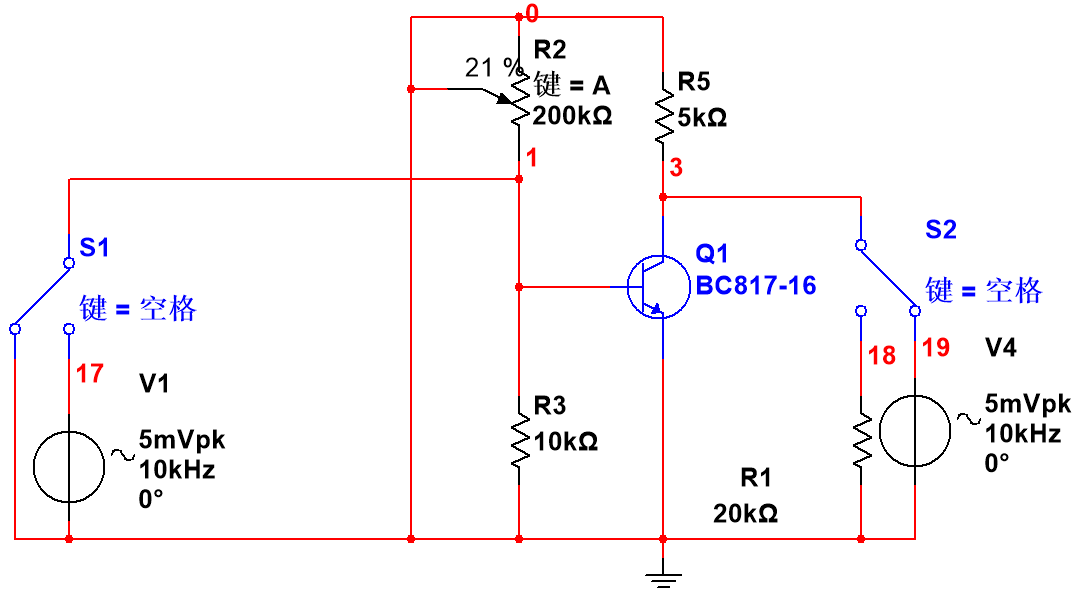
\includegraphics[width=0.8\linewidth]{1/RoAC.png}
	\caption{输出交流通路}
	\label{fig:输出交流通路}
\end{figure}

输出电阻理论值为$ R_5 $ ,为\SI{5}{\kohm}。与实验测得数据\SI{4.75911}{\kohm}基本一致。

\section{实验小结}%
\label{sec:\arabic{chapter}实验小结}

单级放大电路是所有放大电路的基础。难度并不算大,但熟练掌握为之后的学习做好了良好
的铺垫。


\chapter{差动放大电路的设计与仿真}%
\label{cha:差动放大电路的设计与仿真}

\section{实验目的}%
\label{sec:\arabic{chapter}实验目的}

\begin{enumerate}
	\item 设计一个带恒流源的差动放大电路,要求空载时的$ A_\mathrm{VD} $大于20;
	\item 给电路输入\SI{10}{\mV}的直流差模小信号,分别测试电路的双端输出的差模增益$ A_\mathrm{VD} $、单端输出的差模增益$ A_\mathrm{VD1} $;
	\item 给电路输入\SI{1}{\V}的直流共模信号,分别测试双端输出的共模增益$ A_\mathrm{VC} $以及单端输出的共模增益$ A_\mathrm{VC1} $值;
	\item 测量差分放大电路的传输特性曲线。
\end{enumerate}

\section{实验要求}%
\label{sec:\arabic{chapter}实验要求}

\begin{Exercise}
	给出自行设计的差分放大电路原理图,测量其空载时的差模增益。
\end{Exercise}

\begin{Answer}
	差分放大电路原理图见图\ref{fig:差动放大电路原理图},空载时的差模增益见表\ref{tab:差分放大电路参数}。
\end{Answer}

\begin{Exercise}
	给出测量双端输出和单端输出差模增益的电路,求出差模增益的值,并说明单端输出时从$ Q_1 $管输出和从$ Q_2 $管输出的不同。
\end{Exercise}

\begin{Answer}
	双端输出和单端输出电路图见\ref{fig:差动放大电路原理图},差模增益见表\ref{tab:差分放大电路参数},不同是符号相反。
\end{Answer}

\begin{Exercise}
	给出测量双端输出和单端输出共模增益的电路。求出共模增益,并计算共模抑制比。
\end{Exercise}

\begin{Answer}
	测量双端输出和单端输出共模增益的电路图见图\ref{fig:输入共模信号}。共模增益、共模抑制比见表\ref{tab:差分放大电路参数}。
\end{Answer}

\begin{Exercise}
	给出电压传输特性曲线,并对曲线进行必要的说明。
\end{Exercise}

\begin{Answer}
	电压传输特性曲线见图\ref{fig:差动放大电路直流传输特性},说明见章节\ref{sub:\arabic{chapter}仿真结果}。
\end{Answer}

\begin{Exercise}
	分析实验结果。
\end{Exercise}

\begin{Answer}
	分析见章节\ref{sec:\arabic{chapter}实验小结}。
\end{Answer}

\section{实验步骤}%
\label{sec:\arabic{chapter}实验步骤}

\subsection{设计电路}%
\label{sub:\arabic{chapter}设计电路}

\begin{figure}[H]
	\centering
	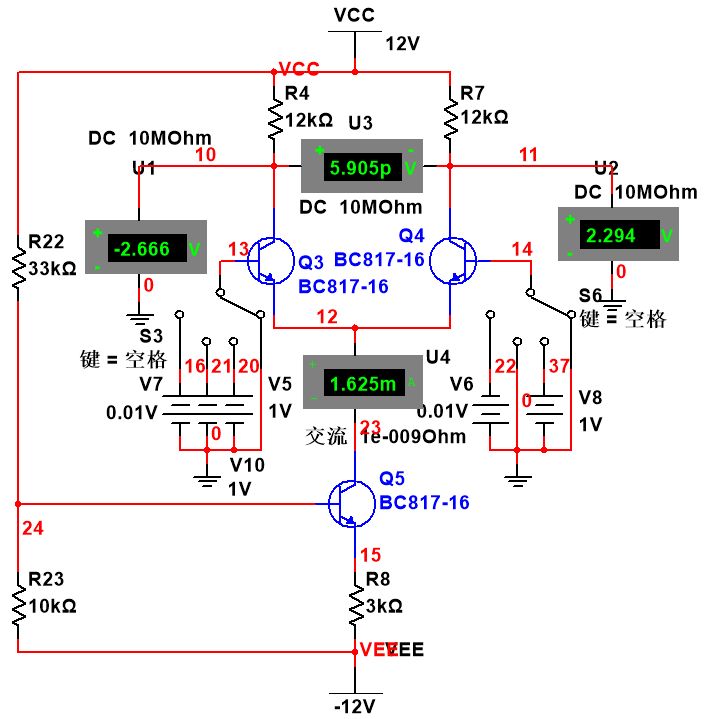
\includegraphics[width=0.8\linewidth]{2/V0.png}
	\caption{差动放大电路原理图}
	\label{fig:差动放大电路原理图}
\end{figure}

如图\ref{fig:差动放大电路原理图}所示,将开关拨到不同位置可以输入不同的信号。输入差模信号见图\ref{fig:输入差模信号},输入共模信号见图\ref{fig:输入共模信号}。

\begin{figure}[H]
	\centering
	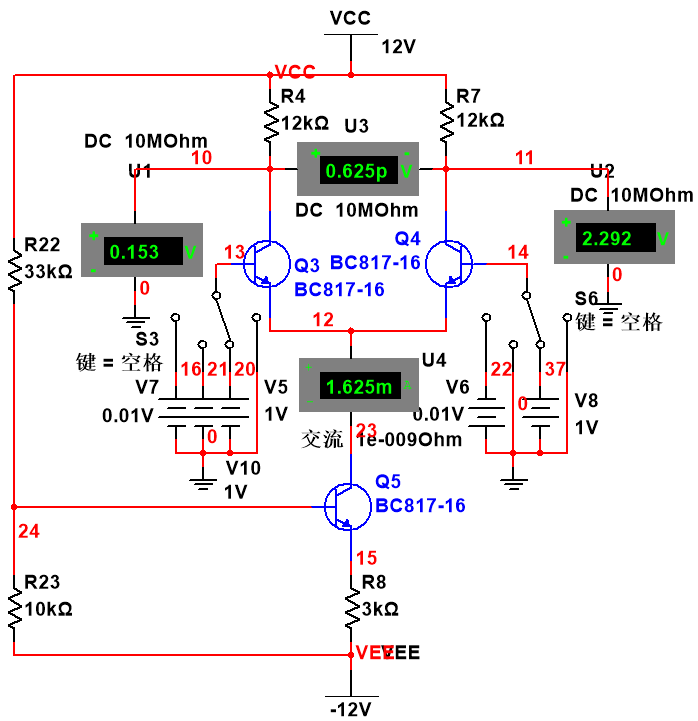
\includegraphics[width=0.8\linewidth]{2/Vc.png}
	\caption{输入差模信号}
	\label{fig:输入差模信号}
\end{figure}

\begin{figure}[H]
	\centering
	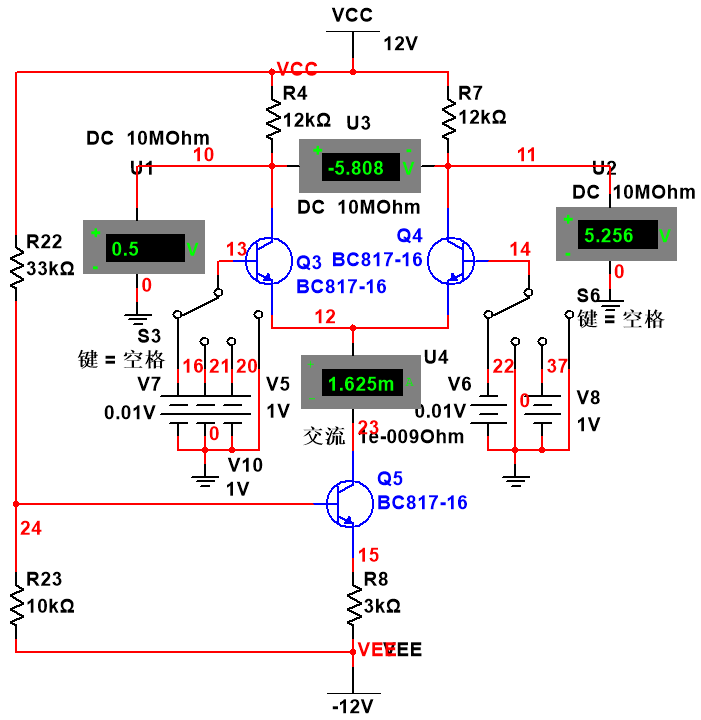
\includegraphics[width=0.8\linewidth]{2/Vd.png}
	\caption{输入共模信号}
	\label{fig:输入共模信号}
\end{figure}

\subsection{指标计算}%
\label{sub:\arabic{chapter}指标计算}

\begin{table}[H]
	\centering
	\caption{差分放大电路参数}
	\label{tab:差分放大电路参数}
	\csvautobooktabular{tab/2/2-1.csv}
\end{table}

\subsection{仿真结果}%
\label{sub:\arabic{chapter}仿真结果}

\begin{figure}[H]
	\centering
	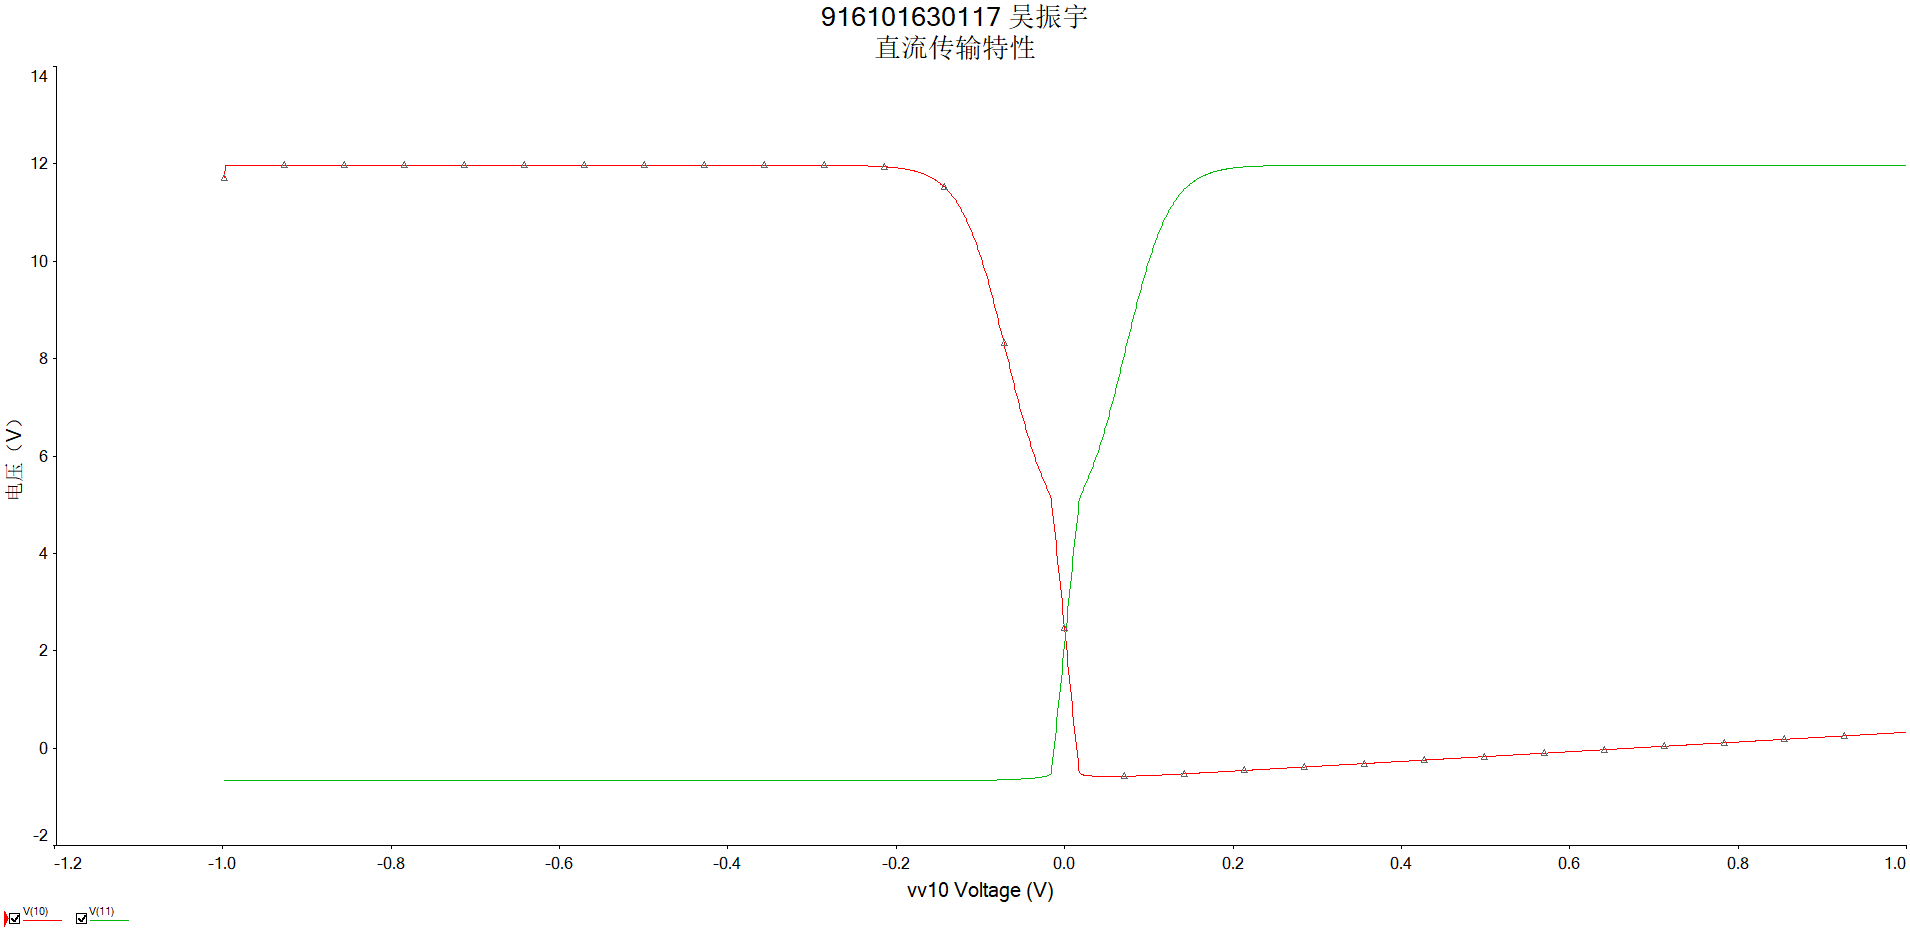
\includegraphics[width=0.8\linewidth]{2/diff.png}
	\caption{差动放大电路直流传输特性}
	\label{fig:差动放大电路直流传输特性}
\end{figure}

差动放大电路直流传输特性曲线见图\ref{fig:差动放大电路直流传输特性},该曲线的对称验证了从$ Q_1 $管输出和从$ Q_2 $管输出的不同是符号相反。

\subsection{误差分析}%
\label{sub:\arabic{chapter}误差分析}

误差分析见表\ref{tab:差动放大电路误差分析},可以看出仿真结果与理论推导相差较小。

\begin{table}[H]
	\centering
	\caption{差动放大电路误差分析}
	\label{tab:差动放大电路误差分析}
	\csvautobooktabular{tab/2/2-2.csv}
\end{table}

\section{实验小结}%
\label{sec:\arabic{chapter}实验小结}

通过此次实验可以看出,差分放大电路对共模信号有着强烈的抑制效果,因为其有这样的特性,所以在现实生活中应用广泛。


\chapter{负反馈放大电路的设计与仿真}%
\label{cha:负反馈放大电路的设计与仿真}

\section{实验目的}%
\label{sec:\arabic{chapter}实验目的}

\begin{enumerate}
	\item 设计一个阻容耦合两级电压放大电路,要求信号源频率\SI{20}{\kHz}(峰值\SI{1}{\mV}),负载电阻\SI{20}{\kohm},电压增益大于100;
	\item 给电路引入电压串联负反馈:
		\begin{enumerate}
			\item 测试负反馈接入前后电路放大倍数、输入、输出电阻和频率特性;
			\item 改变输入信号幅度,观察负反馈对电路非线性失真的影响。
		\end{enumerate}
\end{enumerate}

\section{实验要求}%
\label{sec:\arabic{chapter}实验要求}

\begin{Exercise}
	给出引入电压串联负反馈电路的实验接线图。
\end{Exercise}

\begin{Answer}
	电压串联负反馈电路实验接线图见图\ref{fig:两级闭环放大电路}。
\end{Answer}

\begin{Exercise}
	给出负反馈接入前后电路的放大倍数、输入电阻、输出电阻,并验证$ A_\mathrm{F}\approx\dfrac{1}{F} $。
\end{Exercise}

\begin{Answer}
	负反馈接入前后电路的参数见表\ref{tab:反馈前后指标变化},验证见章节\ref{ssub:放大倍数}。
\end{Answer}

\begin{Exercise}
	给出负反馈接入前后电路的频率特性和$ f_\mathrm{L} $、$ f_\mathrm{H} $值,以及输出开始出现失真时的输入信号幅度。
\end{Exercise}

\begin{Answer}
	负反馈接入前后电路的参数和输出开始出现失真时的输入信号幅度见表\ref{tab:反馈前后指标变化}。
\end{Answer}

\begin{Exercise}
	分析实验结果。
\end{Exercise}

\begin{Answer}
	分析见章节\ref{sec:\arabic{chapter}实验小结}。
\end{Answer}

\section{实验步骤}%
\label{sec:\arabic{chapter}实验步骤}

\subsection{设计电路}%
\label{sub:\arabic{chapter}设计电路}

如图\ref{fig:两级开环放大电路}所示即为两级放大电路且无反馈的原理图。

\begin{figure}[H]
	\centering
	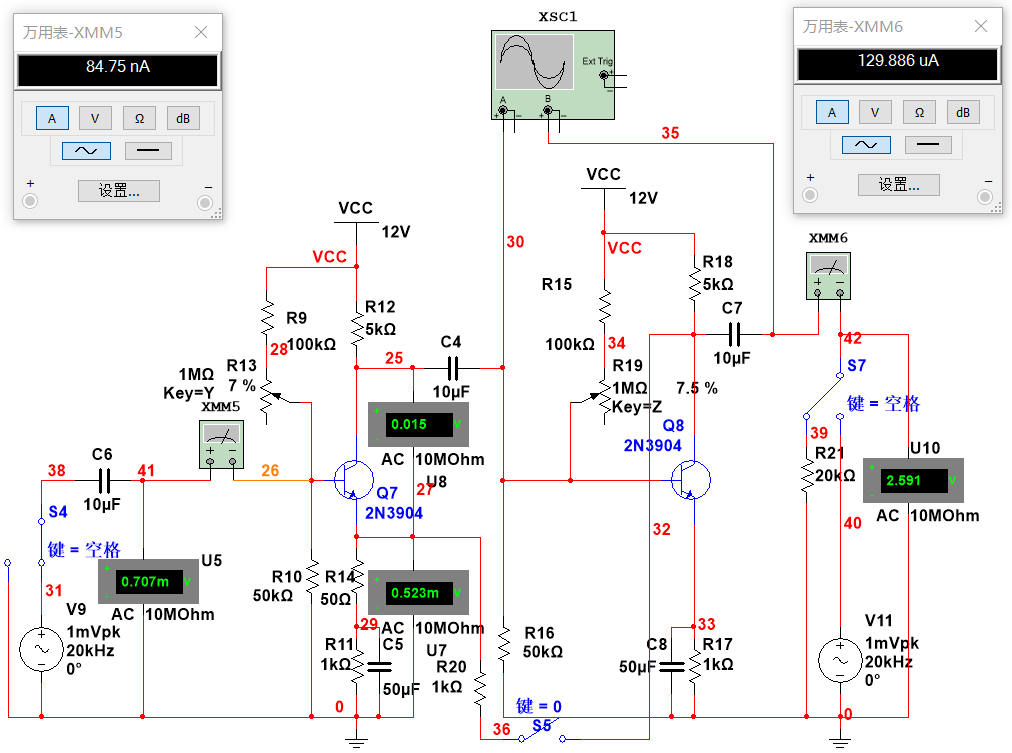
\includegraphics[width = 0.8\linewidth]{3/Ri-open.png}
	\caption{两级开环放大电路}
	\label{fig:两级开环放大电路}
\end{figure}

与单级放大电路类似,采用分压式偏置电路,有效稳定静态工作点。其中$ R_{10},R_9,R_{13} $为第一级电路偏置电阻,$ V_\mathrm{be} = \dfrac{R_{10}}{R9 + R_{13}}V_\mathrm{cc} $,通过调节$ R_{10} $阻值大小可以改变$ V_\mathrm{be} $进而改变静态工作点;$ R_{15}, R_{19}, R_{16} $为第二级电路偏置电阻,$ V_\mathrm{be} = \dfrac{R_{15}}{R_6 + R_{11}}V_\mathrm{cc} $,通过调节$ R_{11} $阻值大小可以改变$ V_\mathrm{be} $进而改变静态工作点;

其中电路放大倍数为第一级、第二级放大倍数之积,为了保证输出信号不失真,因此在第一级电路中加上电阻$ R_{14} $减小第一级放大倍数。由于$ R_{14} $在发射极上,因此交流通路中会阻值等于放大倍数乘以$ R_{14} $,大大减小放大倍数,因此$ R_{14} $不能过大。

如图\ref{fig:两级闭环放大电路}所示即为两级放大电路且有反馈的原理图。

\begin{figure}[H]
	\centering
	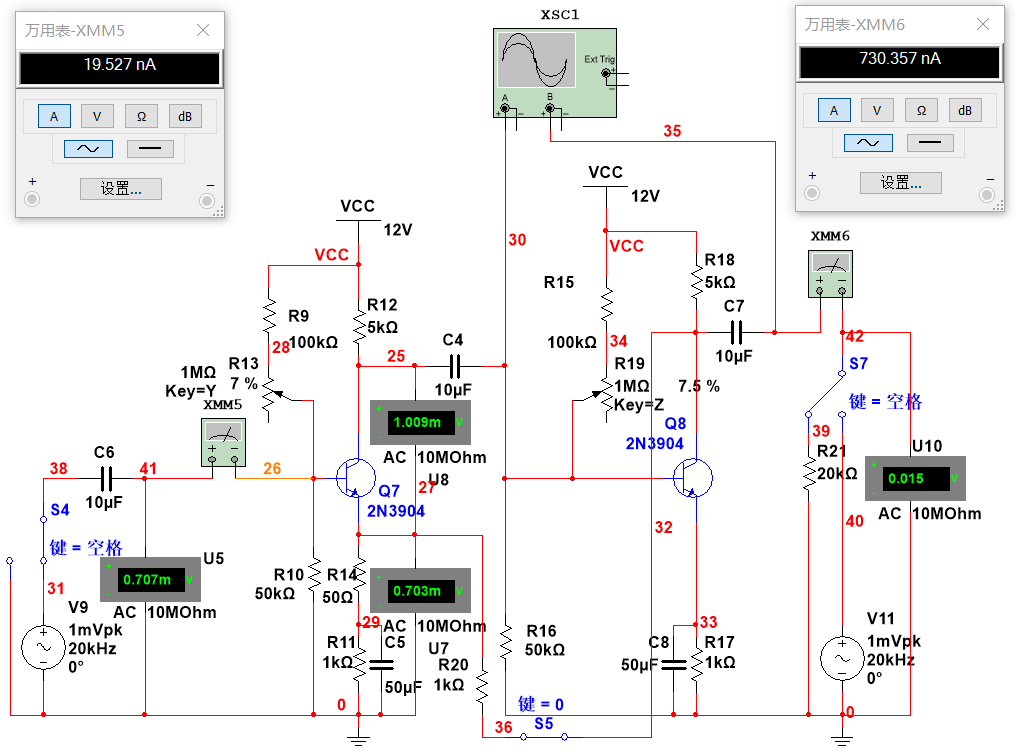
\includegraphics[width = 0.8\linewidth]{3/Ri-close.png}
	\caption{两级闭环放大电路}
	\label{fig:两级闭环放大电路}
\end{figure}

其中反馈电阻为$ R_{20} $,采用电压串联负反馈的方式。为了引入深度负反馈,一般$ R_{20} $阻值为发射极总阻值之和左右。

深度负反馈的主要标志是电路净输入量为0,因此只需测量$ V_\mathrm{b} $、$ V_\mathrm{e} $电压,两者数值相近即$ V_\mathrm{be} $输入量近似为零。

\subsection{指标计算}%
\label{sub:\arabic{chapter}指标计算}

\begin{table}[H]
	\centering
	\caption{两级放大电路参数}
	\label{tab:两级放大电路参数}
	\csvautobooktabular{tab/3/3-1.csv}
\end{table}

\begin{table}[H]
	\centering
	\caption{反馈前后指标变化}
	\label{tab:反馈前后指标变化}
	\csvautobooktabular{tab/3/3-2.csv}
\end{table}

\subsection{仿真结果}%
\label{sub:\arabic{chapter}仿真结果}

\subsubsection{两级放大电路输入电阻}%
\label{ssub:两级放大电路输入电阻}

输入电阻测量原理图如图\ref{fig:两级闭环放大电路}所示,即断开负载电阻,在输入端加入信号源。

采用交流分析法测量输入电阻,由图\ref{fig:两级开环放大电路}可知无反馈时输入电阻为\SI{8.342}{\kohm}。

比较反馈接入前后输入电阻的变化可知电压串联负反馈增大了输入电阻,有利于电路从电压源中获得更大的电压输入,提高电源效率。

\subsubsection{两级放大电路输出电阻}%
\label{ssub:两级放大电路输出电阻}

\begin{figure}[H]
	\centering
	\begin{subfigure}[H]{.7\linewidth}
		\centering
		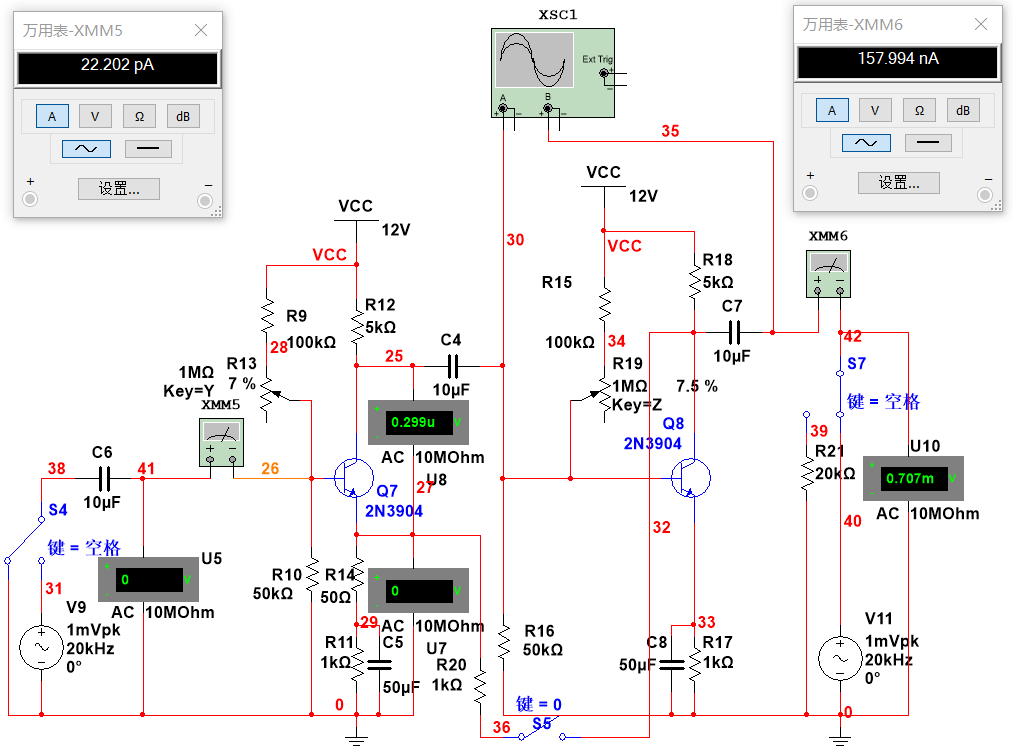
\includegraphics[width=\linewidth]{3/Ro-open.png}
		\caption{两级开环放大电路输出电阻}
		\label{fig:两级开环放大电路输出电阻}
	\end{subfigure}
	\quad
	\begin{subfigure}[H]{.7\linewidth}
		\centering
		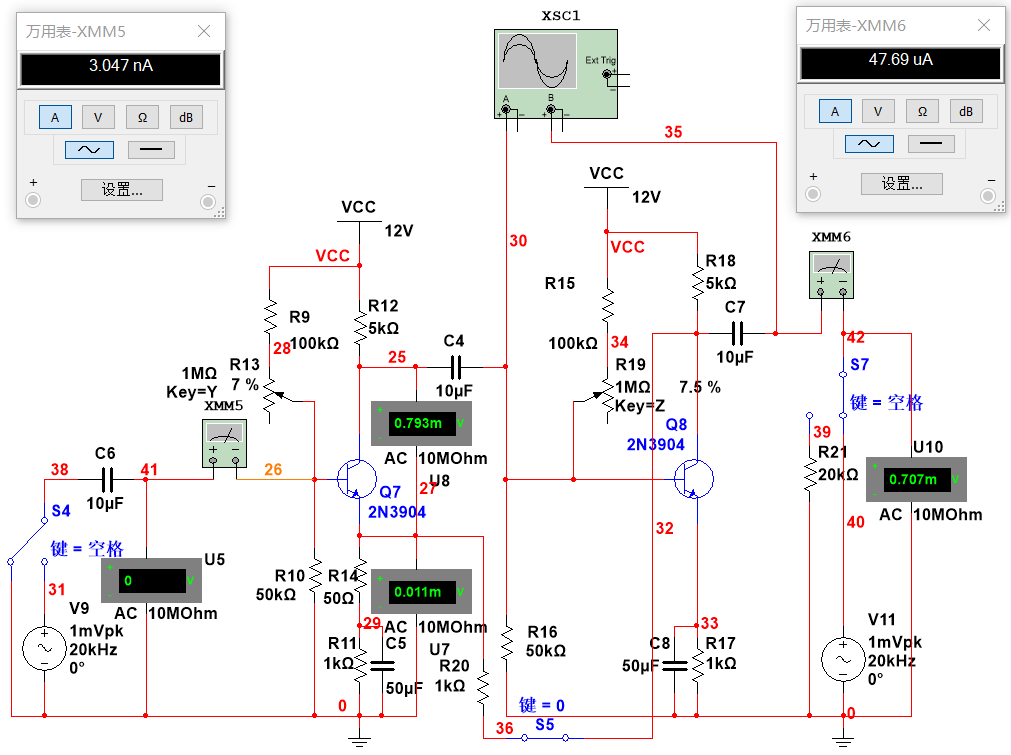
\includegraphics[width=\linewidth]{3/Ro-close.png}
		\caption{两级闭环放大电路输出电阻}
		\label{fig:两级闭环放大电路输出电阻}
	\end{subfigure}
	\caption{两级放大电路输出电阻}
	\label{fig:两级放大电路输出电阻}
\end{figure}

输出电阻测量原理图如图\subref{fig:两级闭环放大电路输出电阻}所示,即短路输入端电压源,断开负载电阻,并在输出端加入信号源。

采用交流分析法测量输出电阻,由图\subref{fig:两级开环放大电路输出电阻}可知无反馈时输出电阻为\SI{16.399}{\kohm}。

比较反馈接入前后输出电阻的变化可知电压串联负反馈减小了输出电阻,提高了负载功率。

\subsubsection{频率特性}%
\label{ssub:频率特性}

由图\ref{fig:两级开环放大电路}可知中频增益\SI{3664.781}{\dB},上下界频率响应对应增益为\SI{3663.781}{\dB},对应上界频率\SI{166.7390}{\kHz},下界频率\SI{97.4882}{\Hz}。

由图\ref{fig:两级闭环放大电路}可知中频增益\SI{21.216}{\dB},上下界频率响应对应增益为\SI{18.216}{\dB},对应上界频率\SI{27153.4}{\kHz},下界频率\SI{23.3005}{\Hz}。

由图\ref{fig:两级开环放大电路}、\ref{fig:两级闭环放大电路}对比可知,负反馈虽然减小了放大倍数,但展宽了通频带。

\begin{figure}[H]
	\centering
	\begin{subfigure}[H]{.8\linewidth}
		\centering
		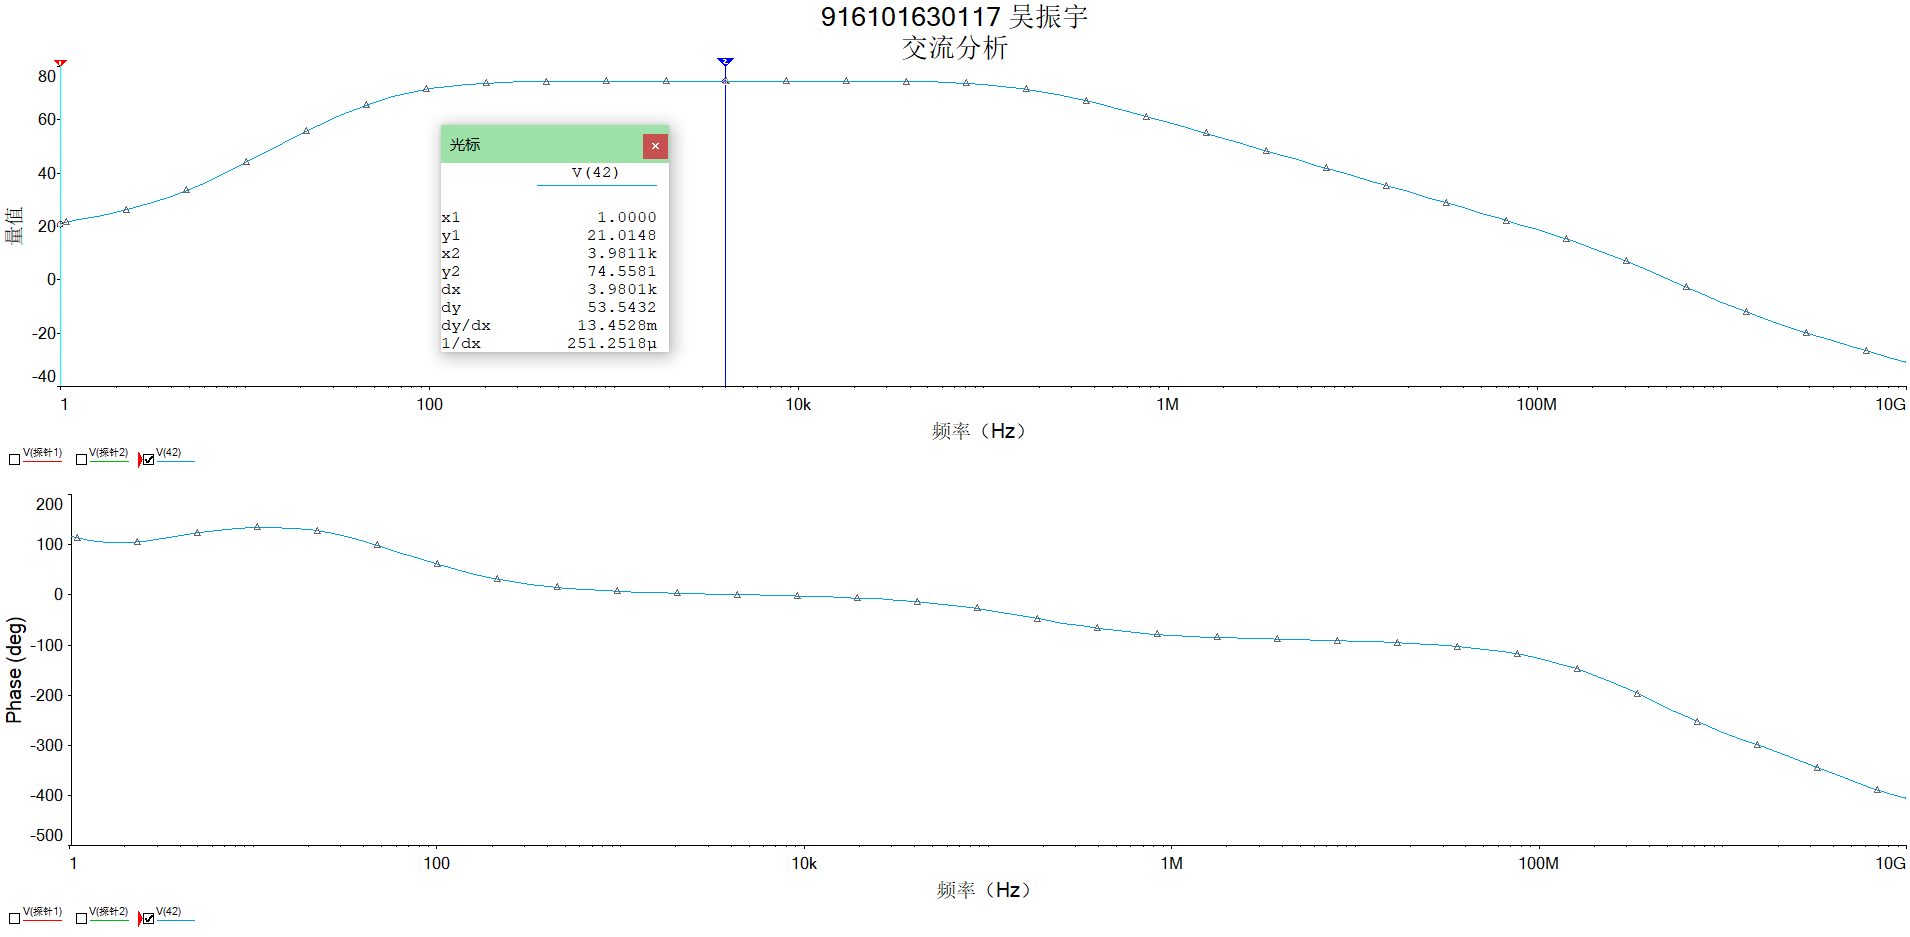
\includegraphics[width=\linewidth]{3/f-open.png}
		\caption{两级开环放大电路放大系数最高点}
		\label{fig:两级开环放大电路放大系数最高点}
	\end{subfigure}
	\quad
	\begin{subfigure}[H]{.8\linewidth}
		\centering
		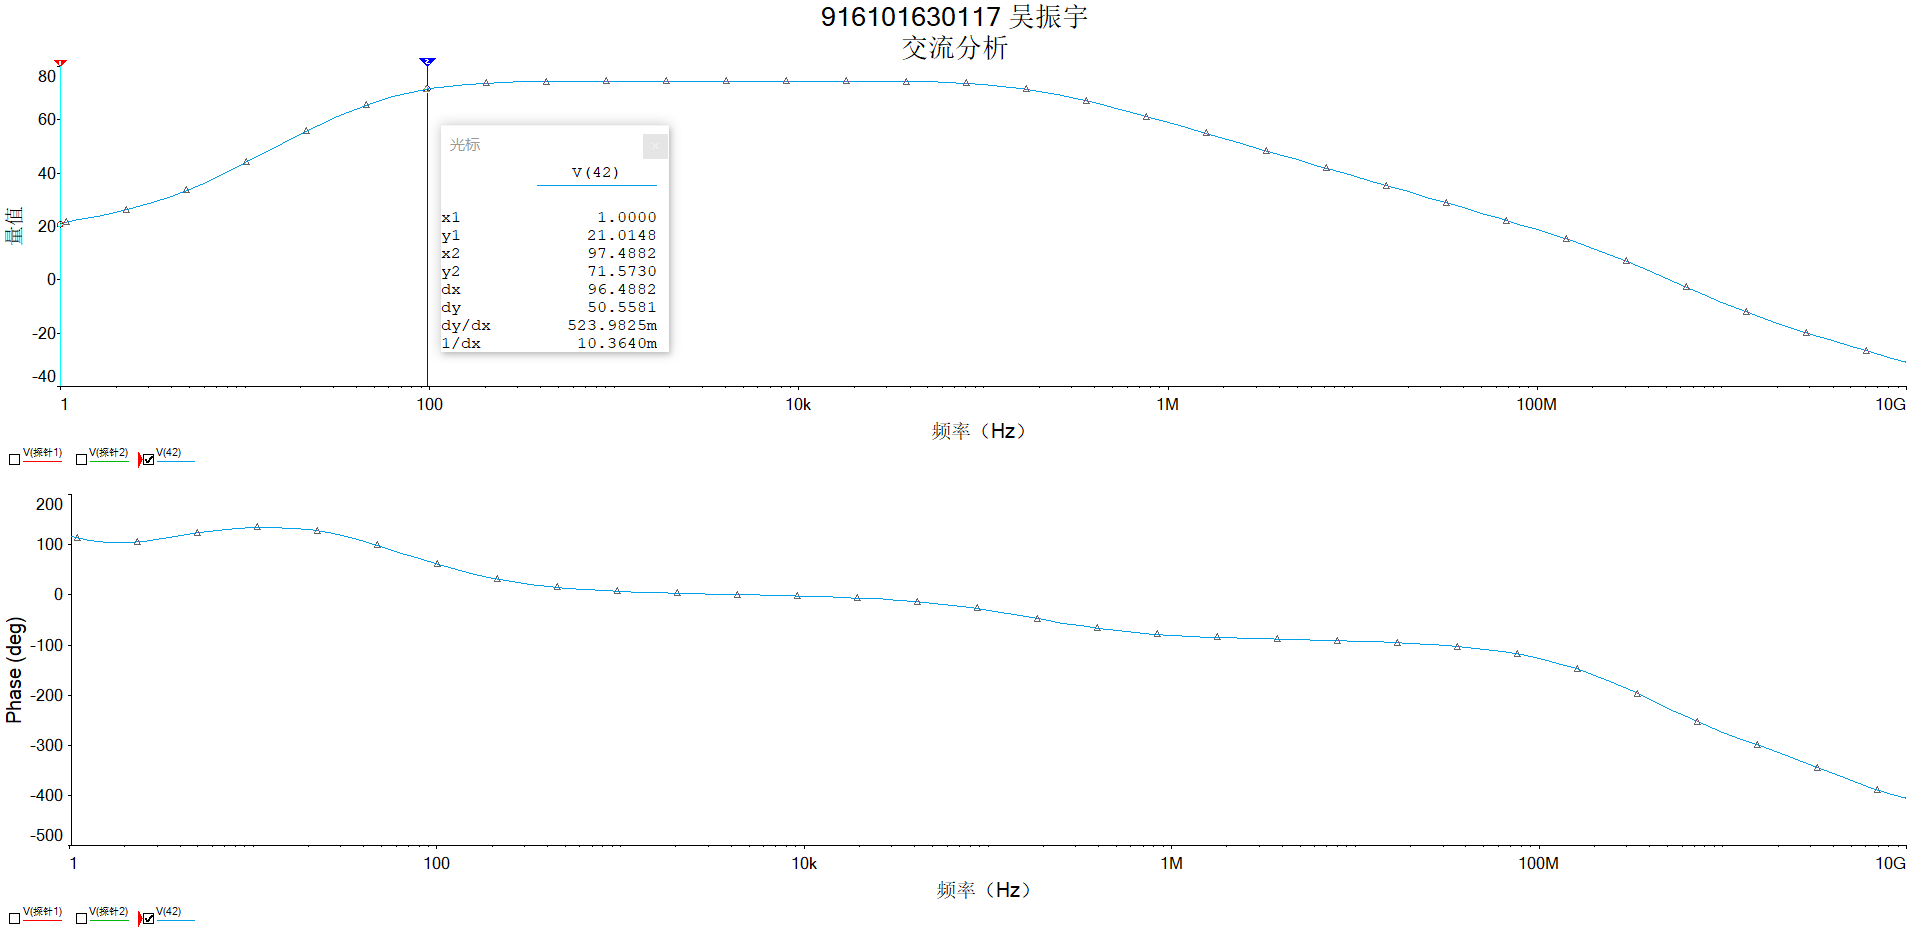
\includegraphics[width = 0.8\linewidth]{3/fL-open.png}
		\caption{两级开环放大电路下截止点}
		\label{fig:两级开环放大电路下截止点}
	\end{subfigure}
	\quad
	\begin{subfigure}[H]{.8\linewidth}
		\centering
		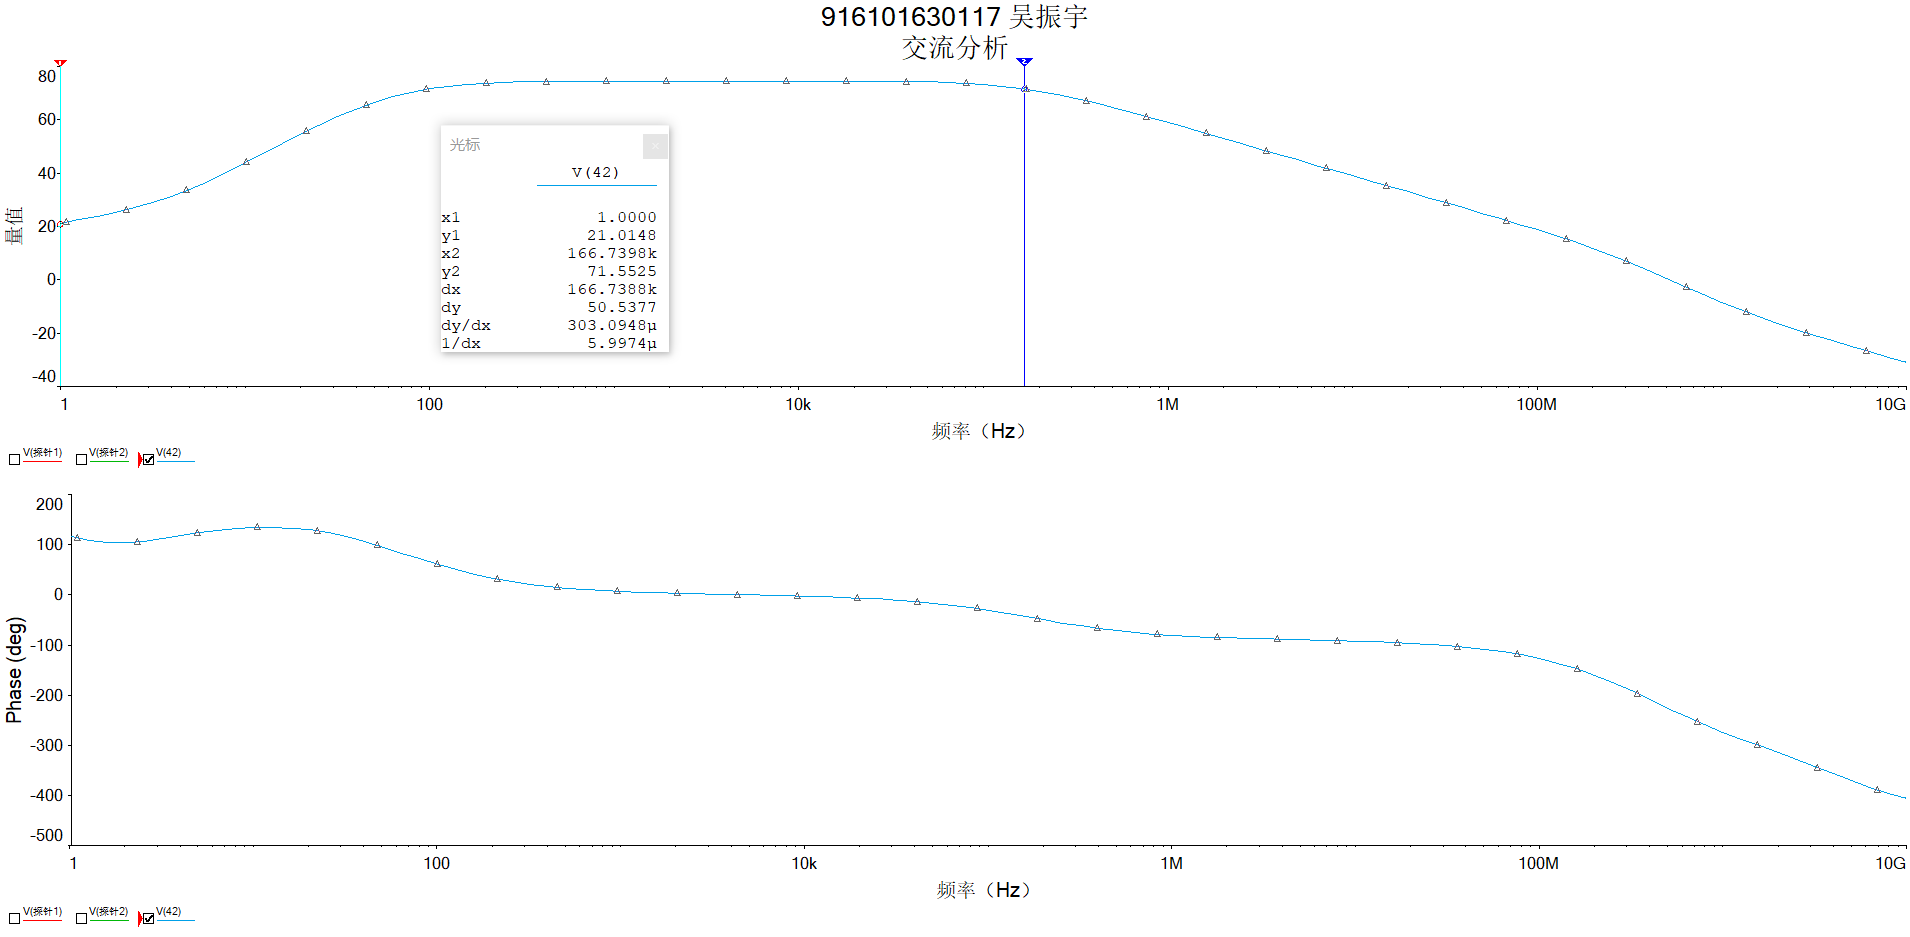
\includegraphics[width=\linewidth]{3/fH-open.png}
		\caption{两级开环放大电路上截止点}
		\label{fig:两级开环放大电路上截止点}
	\end{subfigure}
	\caption{两级开环放大电路}
	\label{fig:两级开环放大电路}
\end{figure}

\begin{figure}[H]
	\centering
	\begin{subfigure}[H]{.8\linewidth}
		\centering
		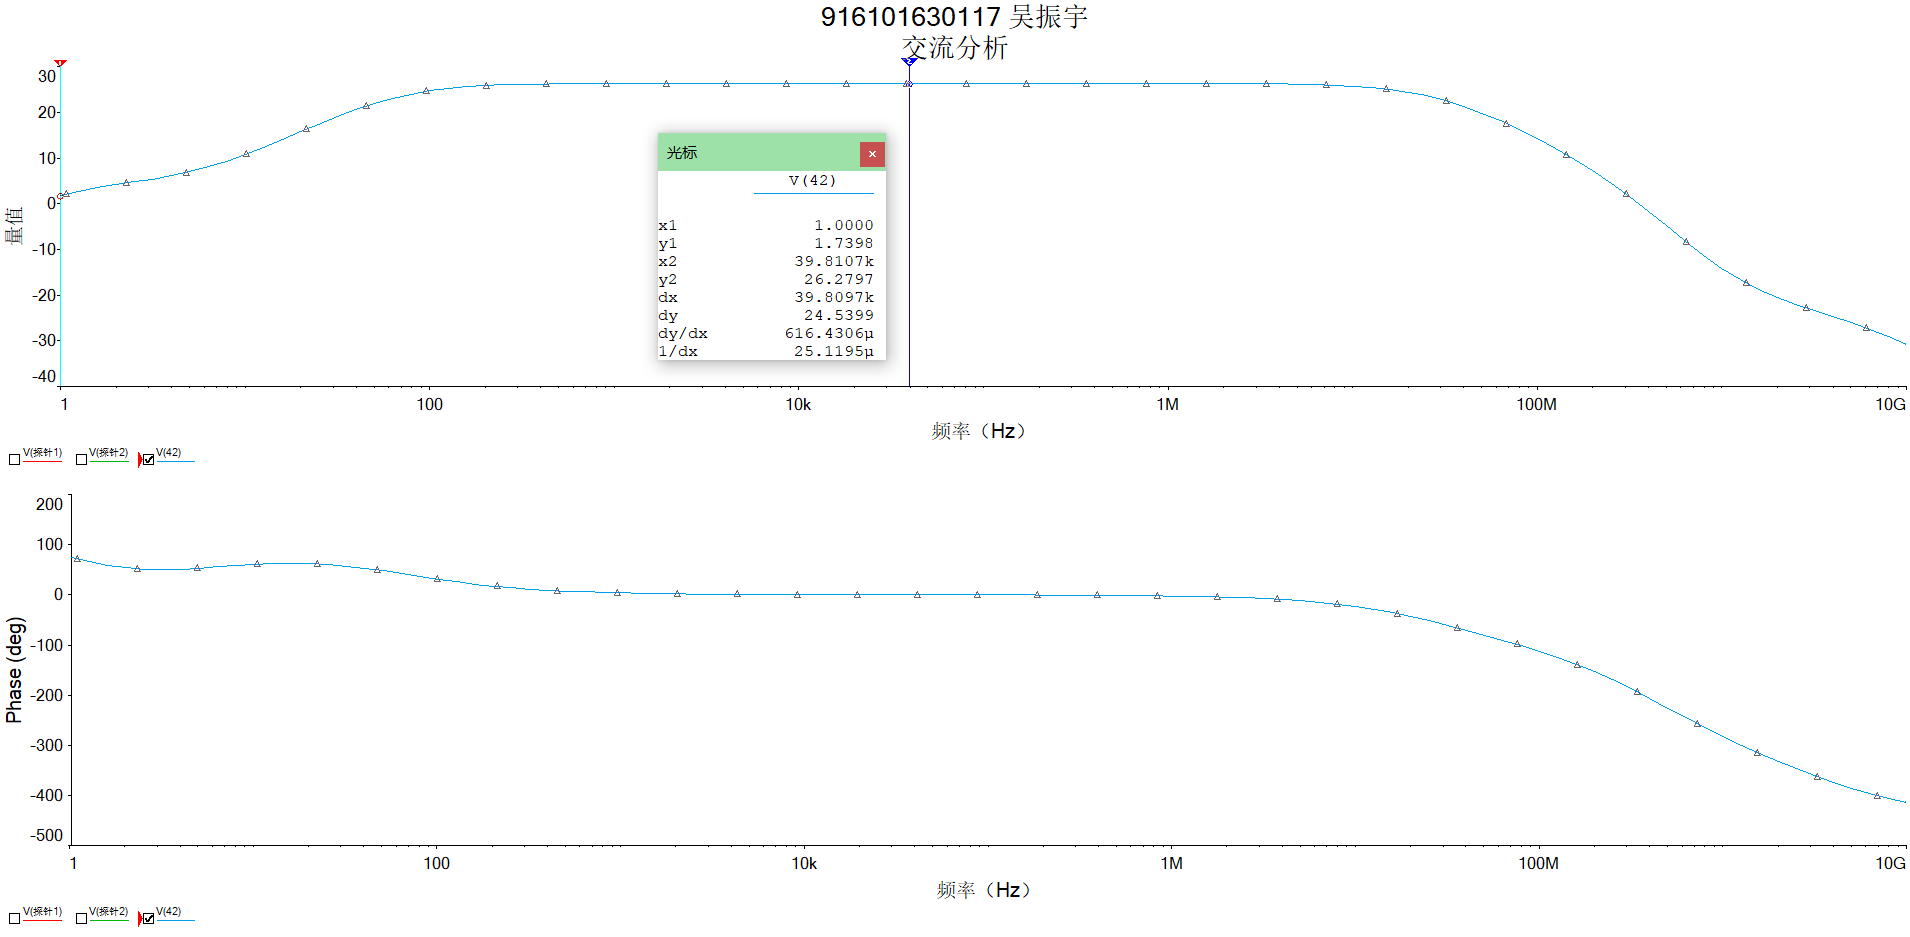
\includegraphics[width=\linewidth]{3/f-close.png}
		\caption{两级闭环放大电路放大系数最高点}
		\label{fig:两级闭环放大电路放大系数最高点}
	\end{subfigure}
	\quad
	\begin{subfigure}[H]{.8\linewidth}
		\centering
		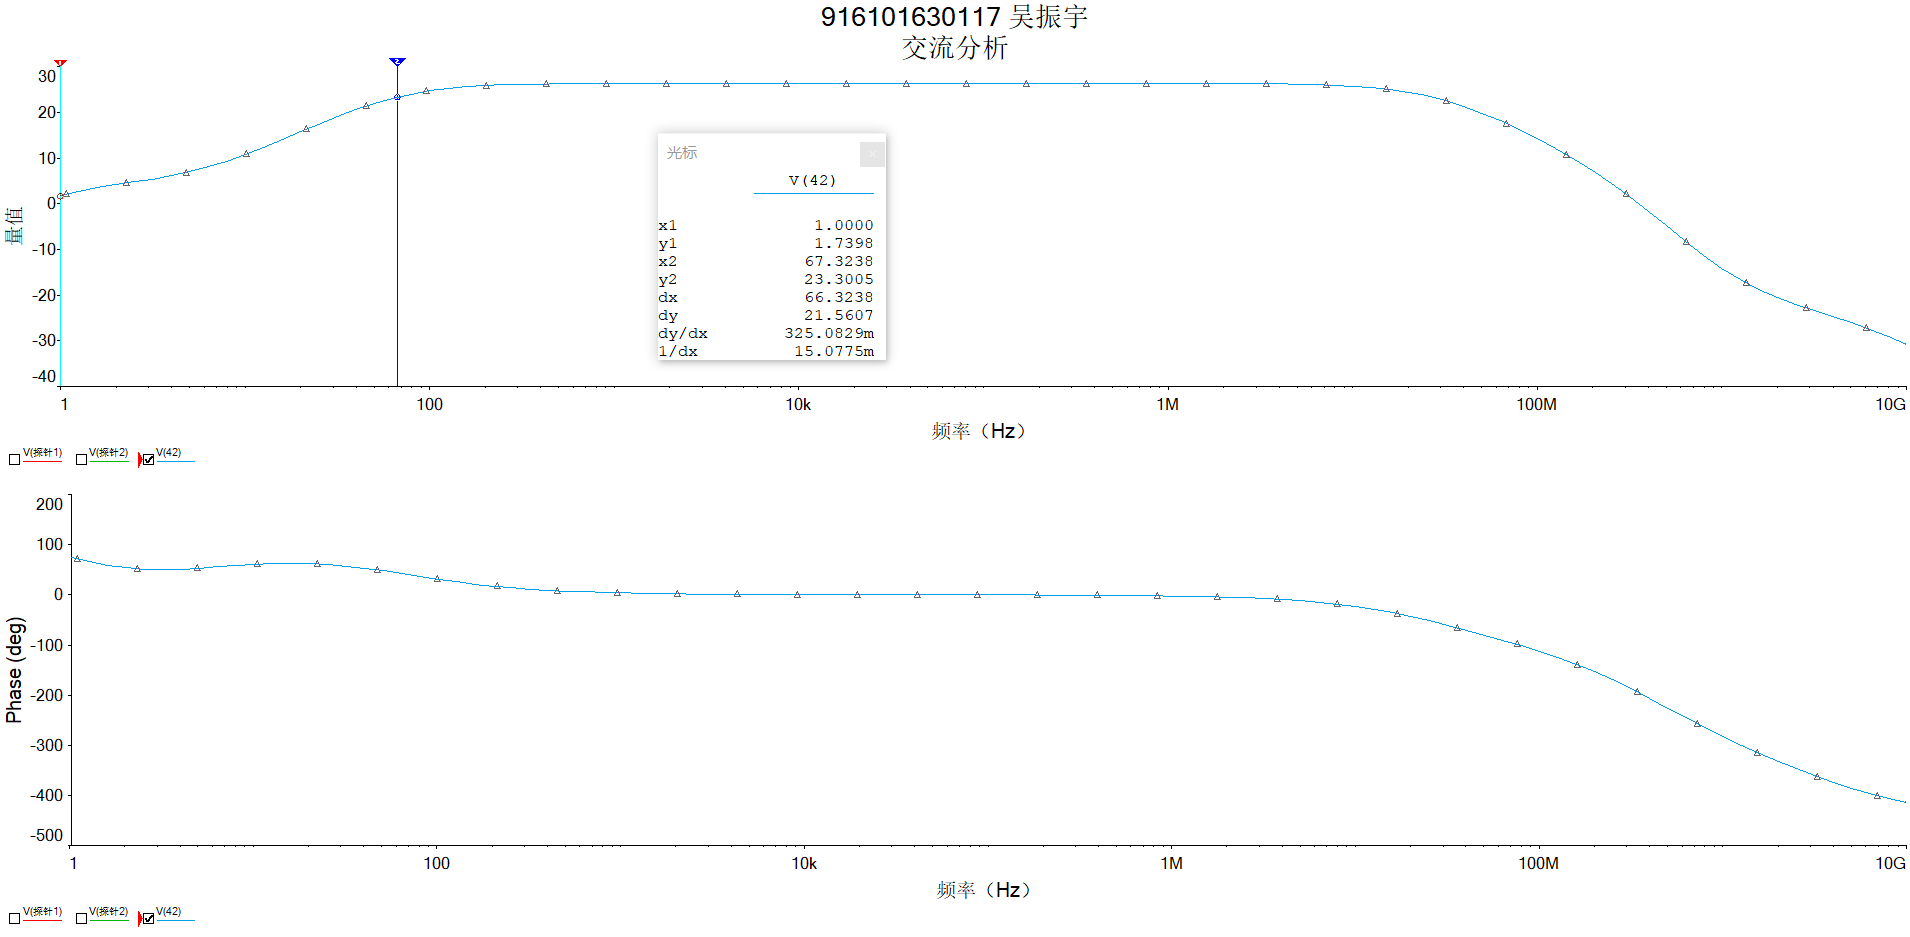
\includegraphics[width = 0.8\linewidth]{3/fL-close.png}
		\caption{两级闭环放大电路下截止点}
		\label{fig:两级闭环放大电路下截止点}
	\end{subfigure}
	\quad
	\begin{subfigure}[H]{.8\linewidth}
		\centering
		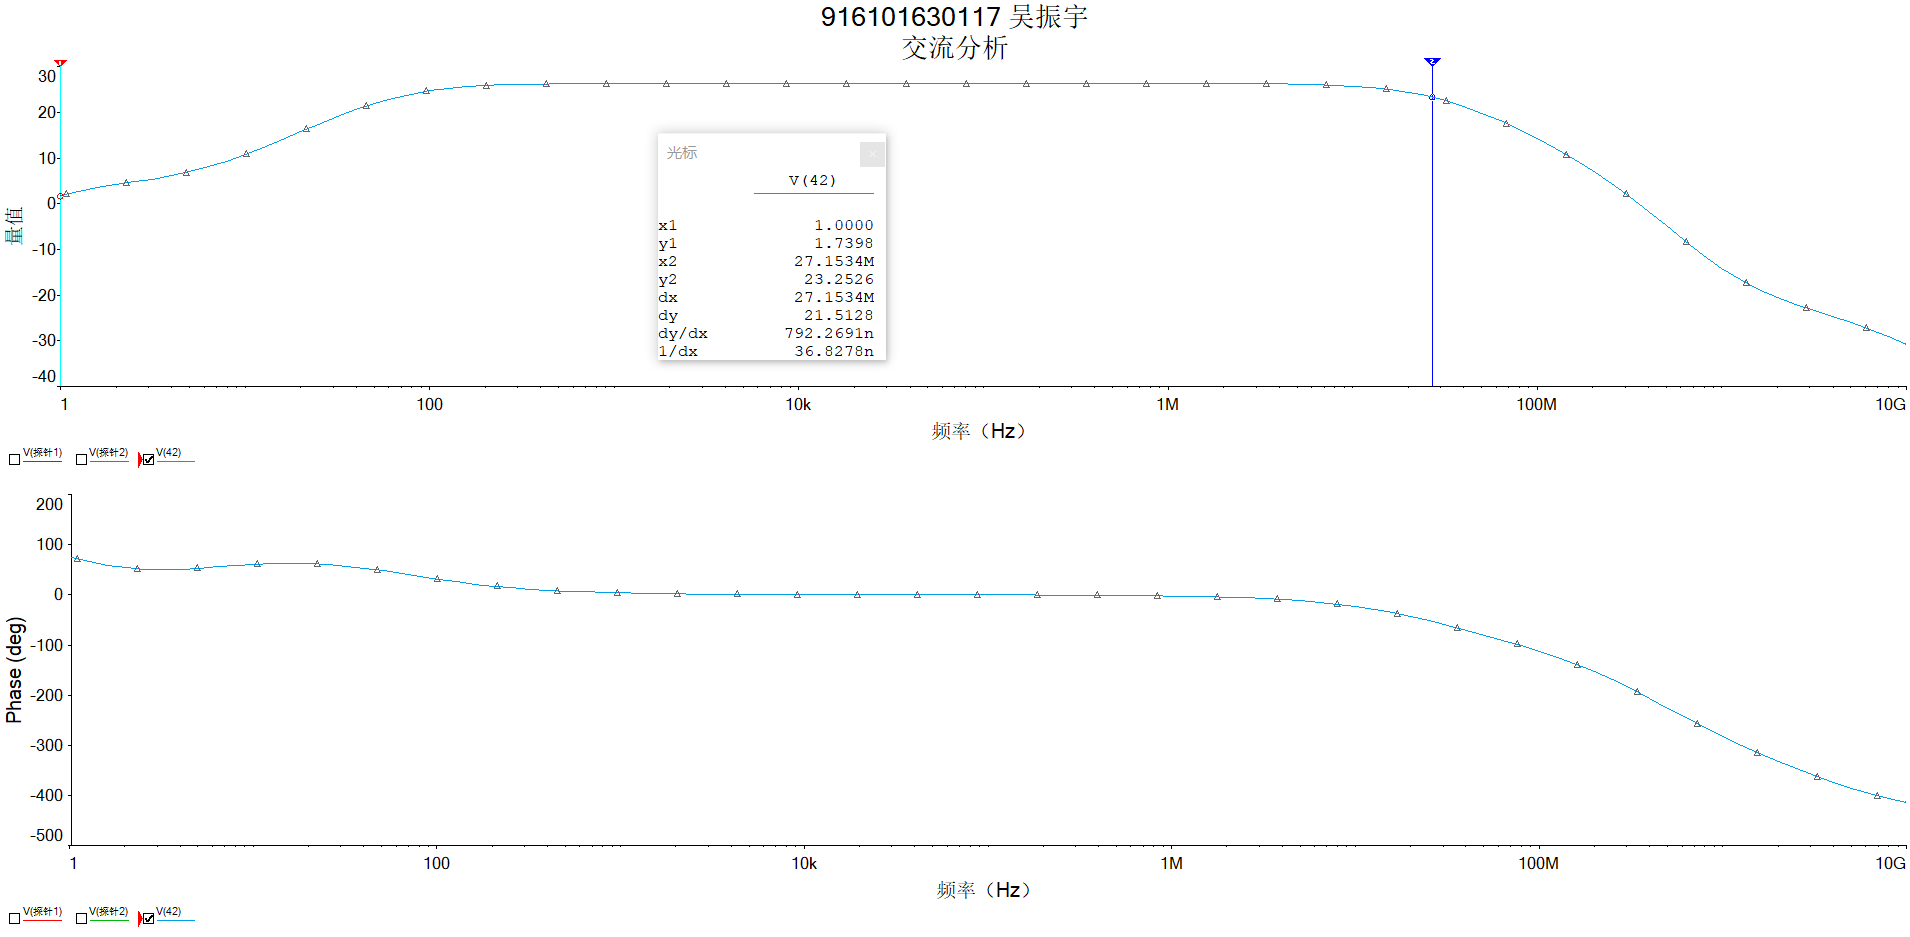
\includegraphics[width=\linewidth]{3/fH-close.png}
		\caption{两级闭环放大电路上截止点}
		\label{fig:两级闭环放大电路上截止点}
	\end{subfigure}
	\caption{两级闭环放大电路}
	\label{fig:两级闭环放大电路}
\end{figure}

\subsubsection{波形失真}%
\label{ssub:波形失真}

\begin{figure}[H]
	\centering
	\begin{subfigure}[H]{.7\linewidth}
		\centering
		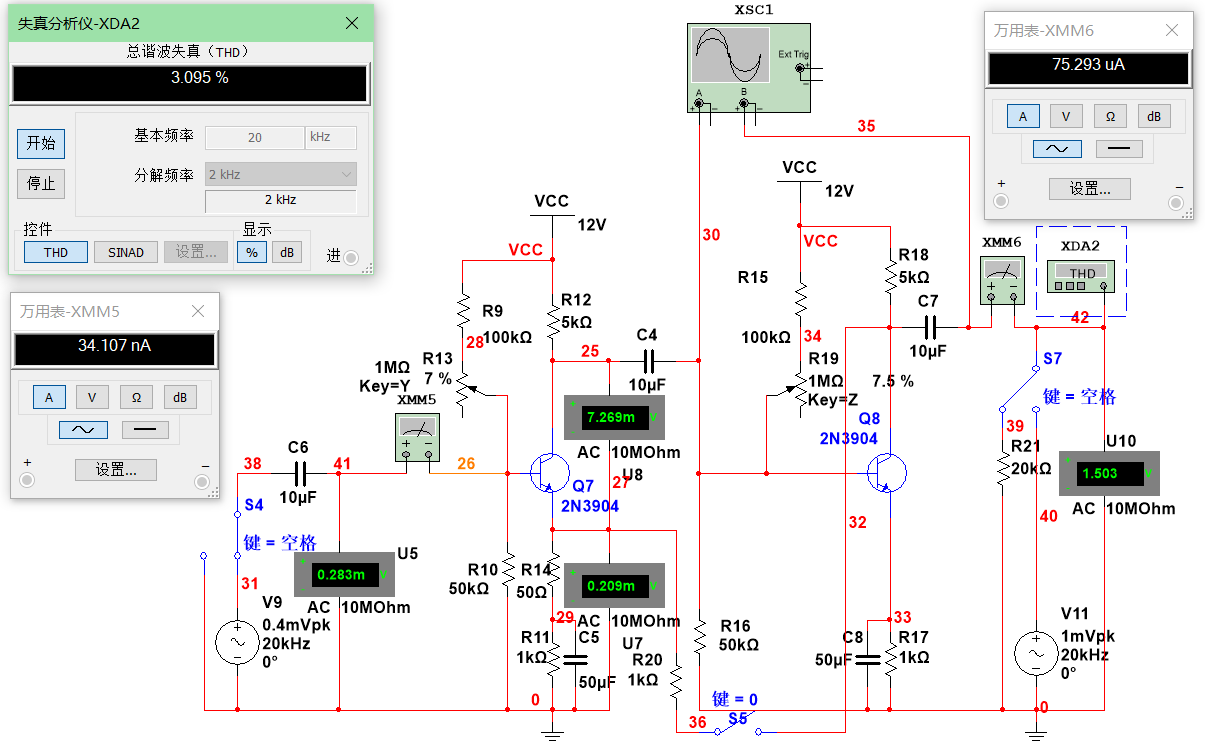
\includegraphics[width=\linewidth]{3/distortion-open.png}
		\caption{两级开环放大电路波形失真}
		\label{fig:两级开环放大电路波形失真}
	\end{subfigure}
	\quad
	\begin{subfigure}[H]{.7\linewidth}
		\centering
		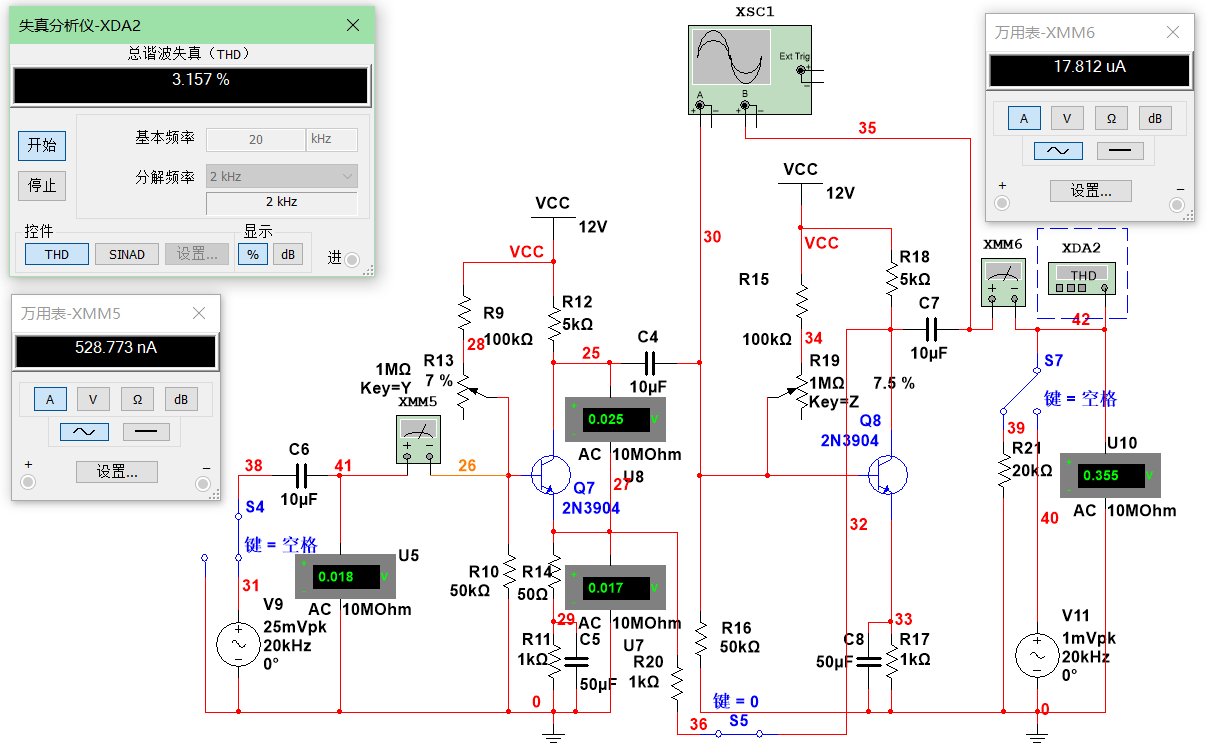
\includegraphics[width=\linewidth]{3/distortion-close.png}
		\caption{两级闭环放大电路波形失真}
		\label{fig:两级闭环放大电路波形失真}
	\end{subfigure}
	\caption{两级放大电路波形失真}
	\label{fig:两级放大电路波形失真}
\end{figure}

未接入反馈时如图\subref{fig:两级开环放大电路波形失真}所示,峰值为\SI{1}{\V}左右,正半周波峰略低于负半轴波峰,这是由于输出特性曲线中靠近截止区时曲线略有上移,而引起的非线性失真。

接入反馈时如图\subref{fig:两级闭环放大电路波形失真}所示,峰值为\SI{1}{\V}左右,正半周波峰几乎等于负半轴波峰,这是由于反馈网络的存在使$ X_\mathrm{i},X_\mathrm{f} $叠加后的输入量矫正了基本放大器的非线性失真。

由对比可知反馈网络对非线性失真具有改善作用。

\subsection{误差分析}%
\label{sub:\arabic{chapter}误差分析}

\subsubsection{放大倍数}%
\label{ssub:放大倍数}

有反馈情况下放大倍数约为21.216倍,反馈电阻值$ R_{20} = \SI{1}{\kohm} $,放大倍数理论值为$ 1 + \dfrac{R_{20}}{R_{14}} = 21 $,与实验结果相吻合。

\section{实验小结}%
\label{sec:\arabic{chapter}实验小结}

本次实验验证了$ A_\mathrm{F}\approx\dfrac{1}{F} $以及反馈电路对开环放大电路的影响。接入反馈电路后,放大倍数变小,电路的稳定性增加,带宽变宽,开始失真时的信号幅度变大。


\chapter{阶梯波发生器的设计与仿真}%
\label{cha:阶梯波发生器的设计与仿真}

\section{实验目的}%
\label{sec:\arabic{chapter}实验目的}

\begin{enumerate}
	\item 设计一个能产生周期性阶梯波的电路,要求阶梯波周期在\SI{30}{\ms}左右,输出电压范围\SI{10}{\V},阶梯个数5个;(注意:电路中均采用模拟、真实器件,不可以选用计数器、555定时器、D/A转换器等数字器件,也不可选用虚拟器件。)对电路进行分段测试和调节,直至输出合适的阶梯波;
	\item 改变电路元器件参数,观察输出波形的变化,确定影响阶梯波电压范围和周期的元器件;
	\item 使用直流扫描分析(DCSweep)工具绘制结型场效应管的转移特性曲线,分析场效应管参数$ I_\mathrm{DSS} $对阶梯波影响的参数。
\end{enumerate}

\section{实验要求}%
\label{sec:\arabic{chapter}实验要求}

\begin{Exercise}
	给出阶梯波发生器实验原理图。
\end{Exercise}

\begin{Answer}
	阶梯波发生器实验原理图见图\ref{fig:阶梯波发生器电路图}。
\end{Answer}

\begin{Exercise}
	介绍电路的工作原理。
\end{Exercise}

\begin{Answer}
	工作原理见章节\ref{sub:\arabic{chapter}仿真结果}。
\end{Answer}

\begin{Exercise}
	给出电路的分段测试波形和最终输出的阶梯波,并回答以下问题:
	\begin{enumerate}
		\item 调节电路中哪些元器件值可以改变阶梯波的周期?
		\item 调节电路中哪些元器件值可以改变阶梯波的输出电压范围?
		\item 调节电路中哪些元器件值可以改变阶梯波的阶梯个数。
	\end{enumerate}
\end{Exercise}

\begin{Answer}
	分段测试波形见图\ref{fig:方波波形图}、\ref{fig:微分电路波形}、\ref{fig:限幅电路波形}、\ref{fig:积分电路波形}、\ref{fig:脉冲波形},最终输出的阶梯波见图\ref{fig:向上阶梯波形}。调节电路中元器件值见章节\ref{sub:\arabic{chapter}指标计算}。
\end{Answer}

\begin{Exercise}
	说明设计和调试过程中出现的问题与解决办法,以及改进和创新性方案。
\end{Exercise}

\begin{Answer}
	设计和调试过程中出现的问题与解决办法见章节\ref{sub:\arabic{chapter}误差分析},改进和创新性方案见章节\ref{ssub:向下阶梯波形}。
\end{Answer}

\section{实验步骤}%
\label{sec:\arabic{chapter}实验步骤}

\subsection{设计电路}%
\label{sub:\arabic{chapter}设计电路}

\begin{figure}[H]
	\centering
	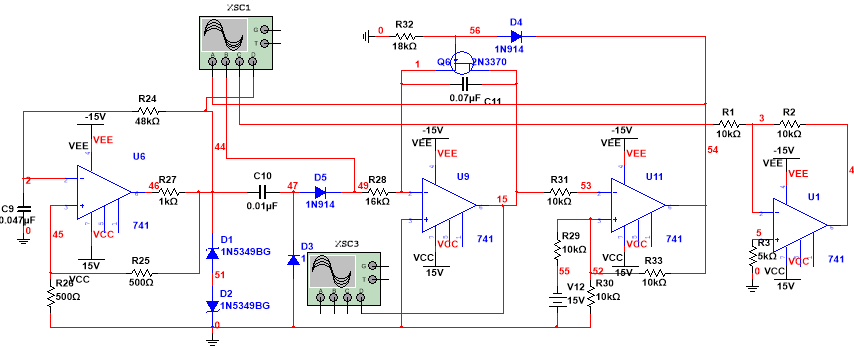
\includegraphics[width=0.8\linewidth]{4/JFET.png}
	\caption{阶梯波发生器电路图}
	\label{fig:阶梯波发生器电路图}
\end{figure}

\subsection{指标计算}%
\label{sub:\arabic{chapter}指标计算}

\begin{enumerate}
	\item 根据方波发生器的周期$ T = 2R_1C_1\ln(1 + 2\dfrac{R_2}{R_4}) $可得,改变$ R_4,C_1,R_1,R_2 $的值可以改变阶梯波的周期。
	\item 根据原理可知,输出电压范围和滞回比较器的门限电压有关。所以改变$ R_7,R_8 $可以改变输出电压。改变滞回比较器的直流电源值也会影响输出电压范围。
	\item 要改变阶梯波的阶梯个数:

		\begin{enumerate}
			\item 可以改变积分的高度,即改变微分电路和积分电路内部元器件参数。使得在一个周期中有更多或者更少的阶梯数;
			\item 改变迟滞比较器的的上下限的值。
		\end{enumerate}
\end{enumerate}

\subsection{仿真结果}%
\label{sub:\arabic{chapter}仿真结果}

\subsubsection{方波发生器}%
\label{ssub:方波发生器}

\begin{wrapfigure}{r}{0.6\linewidth}
	\centering
	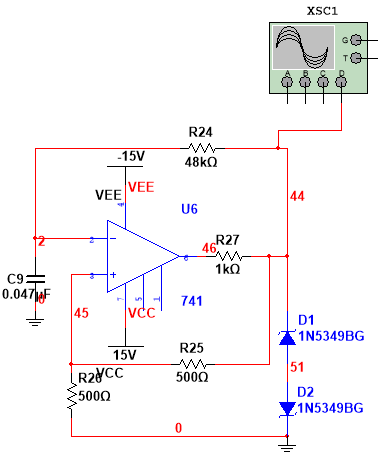
\includegraphics[width=\linewidth]{4/squareJFET.png}
	\caption{方波发生器}
	\label{fig:方波发生器}
\end{wrapfigure}

方波发生器是运放非线性运用,工作原理为当输入端为高电平时通过$ R_\mathrm{f}, C $电路放电直到电容两端电压达到翻转电压,此时运算放大器翻转,输出电压变为负值,此时通过$ R_\mathrm{f}C $电路充电直到翻转电压;方波发生器通过充放电在两种状态中循环切换,形成周期方波。

其中$ D_{1},D_{2} $为稳压管,导通电压\SI{10}{\V},配合$ R_{24} $实现输出电压限幅;

芯片同相输入端接$ R_{25}, R_{26} $,决定了翻转电压$ V_+ = \dfrac{R_{26}}{R_{25}+R_{26}}V_\mathrm{omax} $、$ V_- = \dfrac{R_{26}}{R_{25}+R_{26}}V_\mathrm{omin} $;

芯片反相输入端$ R_{24}, C_9 $组成充放电电路,时间常数为$ \dfrac{1}{R_\mathrm{f}C} $;

周期$ T = 2R_\mathrm{f}C\ln(1 + 2\dfrac{R_2}{R_3}) $为满足五个阶梯波周期为\SI{30}{\ms},因此方波周期为\SI{6}{\ms},构造$ R_{25}, R_{26} $为相同值,$ R_\mathrm{f} = \SI{48}{\kohm} $,$ C = \SI{0.047}{\mu\F} $,满足周期要求。

方波波形图如图\ref{fig:方波波形图}所示。

\begin{figure}[H]
	\centering
	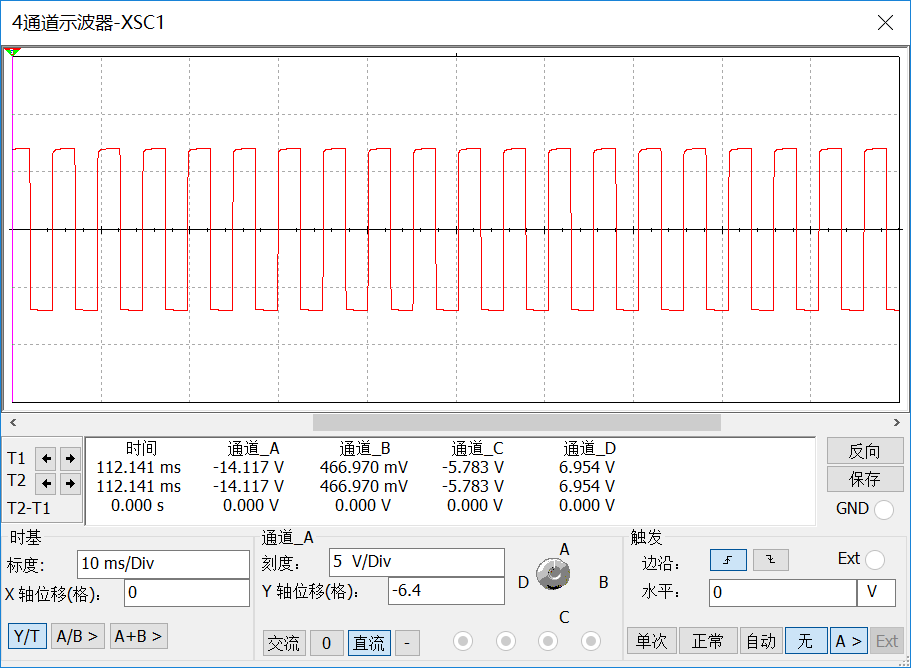
\includegraphics[width = 0.8\linewidth]{4/square.png}
	\caption{方波波形图}
	\label{fig:方波波形图}
\end{figure}

\newpage

\subsubsection{微分电路}%
\label{ssub:微分电路}

\begin{figure}[H]
	\centering
	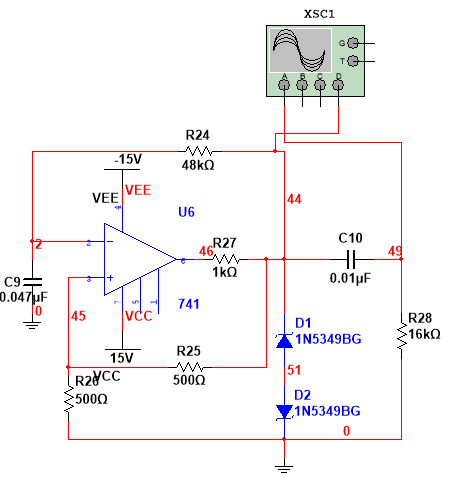
\includegraphics[width=.8\linewidth]{4/diffJFET.png}
	\caption{微分电路}
	\label{fig:微分电路}
\end{figure}

微分电路如图所示,主要是电容$ C_{10}, R_{28} $进行充放电,由于时间常数$ C_{10}R_{28} $比较小因此方波变成了尖脉冲形式,尖脉冲位置都在在方波突变位置。

微分电路波形如图\ref{fig:微分电路波形}所示。

\begin{figure}[H]
	\centering
	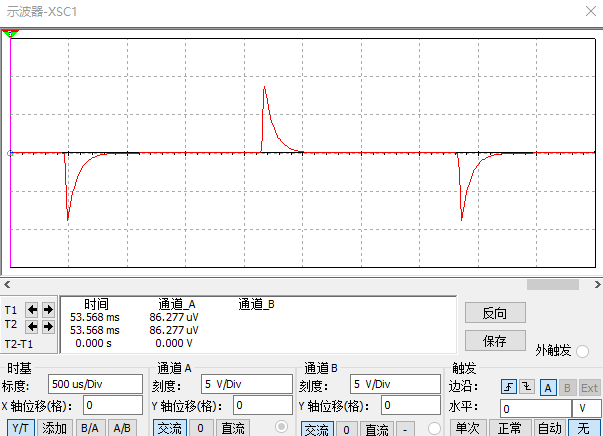
\includegraphics[width=0.8\linewidth]{4/diff.png}
	\caption{微分电路波形}
	\label{fig:微分电路波形}
\end{figure}

\subsubsection{限幅电路}%
\label{ssub:限幅电路}

\begin{figure}[H]
	\centering
	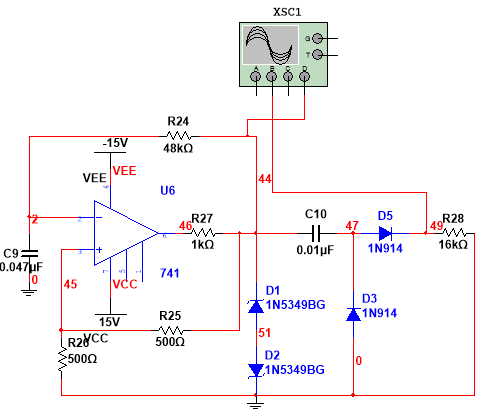
\includegraphics[width=0.8\linewidth]{4/limitJFET.png}
	\caption{限幅电路}
	\label{fig:限幅电路}
\end{figure}

限幅电路如图所示,主要是通过二极管$ D_3, D_5 $完成限幅功能。方波正周期时,$ D_5 $导通,$ C_{10}, R_{28} $构成微分电路形成正向尖脉冲,负周期时$ D_3 $导通、电容直接接地,不产生负周期尖脉冲。因此完成了限幅功能。

限幅波形如图\ref{fig:限幅电路波形}所示。

\begin{figure}[H]
	\centering
	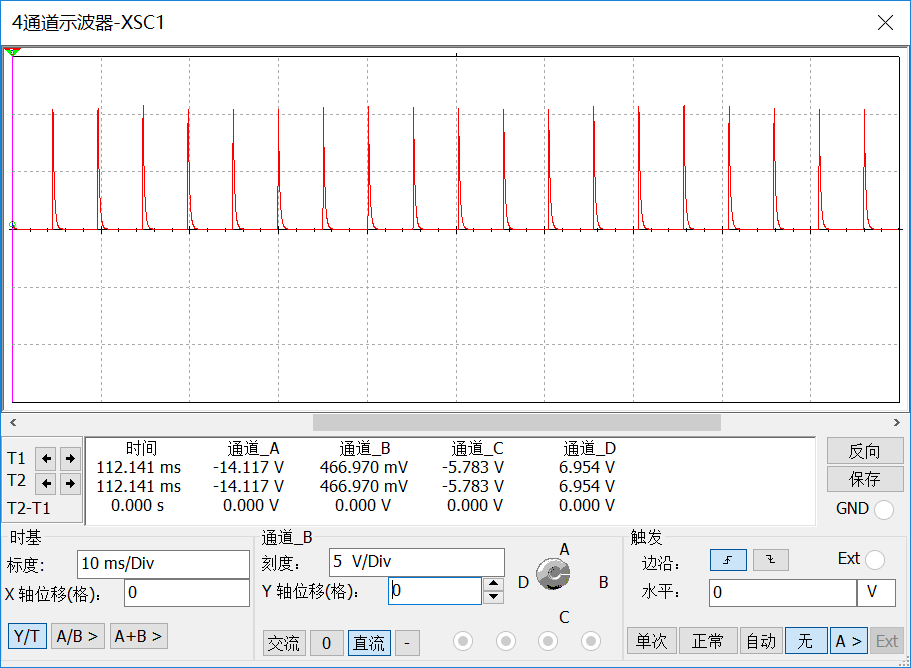
\includegraphics[width = 0.8\linewidth]{4/limit.png}
	\caption{限幅电路波形}
	\label{fig:限幅电路波形}
\end{figure}

\subsubsection{积分电路}%
\label{ssub:积分电路}

\begin{figure}[H]
	\centering
	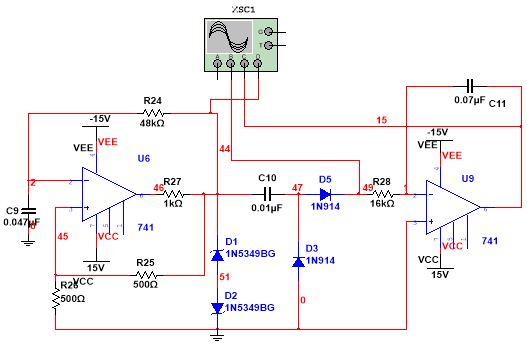
\includegraphics[width=0.8\linewidth]{4/integrateJFET.png}
	\caption{积分电路}
	\label{fig:积分电路}
\end{figure}

积分电路主要由$ R_{28}, C_{11} $以及运放组成。积分电路输入端是尖脉冲,因此积分时间很短,是积分输出波形几乎是发生突变、且在下一个尖脉冲到来之前输出端电压保持不变构成阶梯波的形式。

由于设计要求周期为\SI{}{\ms}级别,因此$ R_{28}C_{11} $单位为\SI{}{\ms}。

根据周期和峰值要求选用$ R_{28} = \SI{16}{\kohm}, C_3 = \SI{0.07}{\mu\F} $。

积分电路波形如图\ref{fig:积分电路波形}所示,上下限为电源电压\SI{15}{\V}左右。

\begin{figure}[H]
	\centering
	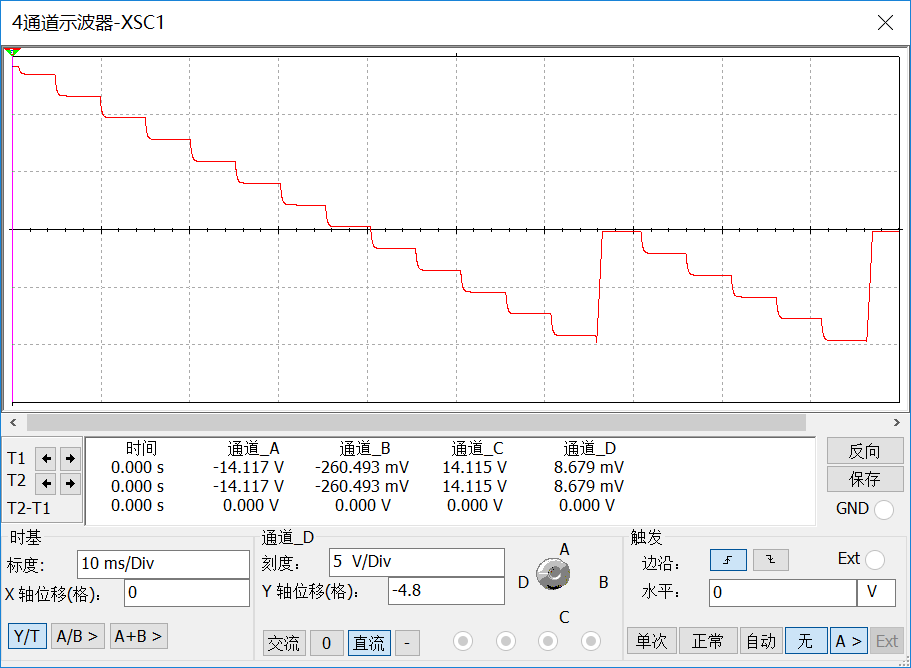
\includegraphics[width = 0.8\linewidth]{4/integrate.png}
	\caption{积分电路波形}
	\label{fig:积分电路波形}
\end{figure}

\subsubsection{比较器及电子开关电路}%
\label{ssub:比较器及电子开关电路}

\begin{figure}[H]
	\centering
	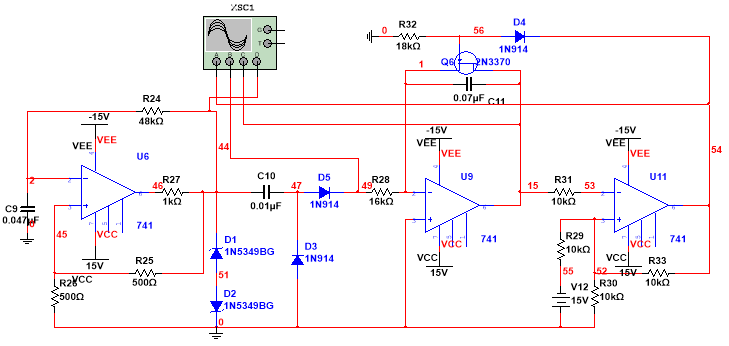
\includegraphics[width=\linewidth]{4/pulseJFET.png}
	\caption{比较器及电子开关电路}
	\label{fig:比较器及电子开关电路}
\end{figure}

比较器及电子开关电路如图\ref{fig:比较器及电子开关电路}所示。

其中比较器为迟滞比较器,主要由运放$ U_{11}, R_{31}, R_{29}, R_{30}, R_{33} $、参考电压$ V_{11} $组成。$ R_{31} $主要是限制输入电流保护运放;$ V_{12} $构成参考电压$ -V_\mathrm{R} $;通过调整$ R_{29}, R_{30}, R_{33} $能够调整门限电压。

电子开关电路由$ D_4 $、MOS管$ U_{11} $组成。当运放$ U_{11} $输出负值时电子开关关断、$ D_4 $不导通,输出回路对方波发生器无影响;当运放$ U_{11} $输出正值时电子开关导通、$ D_4 $也导通。

电路稳定时主要工作原理是反向输入端输入阶梯波,此时大于下门限电压,输出\SI{-15}{\V},此时$ D_4 $导通,场效应管栅极电压为负值,负电压使场效应管处于夹断状态,N沟道场效应管不能导通,同时$ D_4 $截止,比较器对方波发生器无影响;积分器输出电压不断降低,阶梯个数逐渐增加时,反相输入端到达下门限电压后比较器翻转输出\SI{+15}{\V},此时$ D_4 $截止,场效应管栅极电压变为0,场效应管导通,通过电容$ C11 $迅速放电,同时$ D_4 $变为导通,方波发生器输出负值,即比较器翻转时方波发生器输出负值使阶梯波起始波形相同。

由于设计要求5个阶梯波\SI{10}{\V}左右,因此上门限电压选为\SI{0}{\V},下门限电压选为\SI{-10}{\V},由于输出电压为\SI{+-15}{\V},因此选参考电压$ V_\mathrm{R} = \SI{-15}{\V} $,因此下门限电压等于$ \SI{-10}{\V} = \dfrac{V_\mathrm{omin} + V_\mathrm{R}}{3} $,上门限电压$ \SI{0}{\V} = \dfrac{V_\mathrm{omax} + V_\mathrm{R}}{3} $,因此$ R_{29}, R_{30}, R_{33} $均为\SI{10}{\kohm},$ R_{29}\parallel R_{30} $为\SI{5}{\kohm},分压为$ \dfrac{V_\mathrm{o}}{3} $,符合设计要求。

\begin{figure}[H]
	\centering
	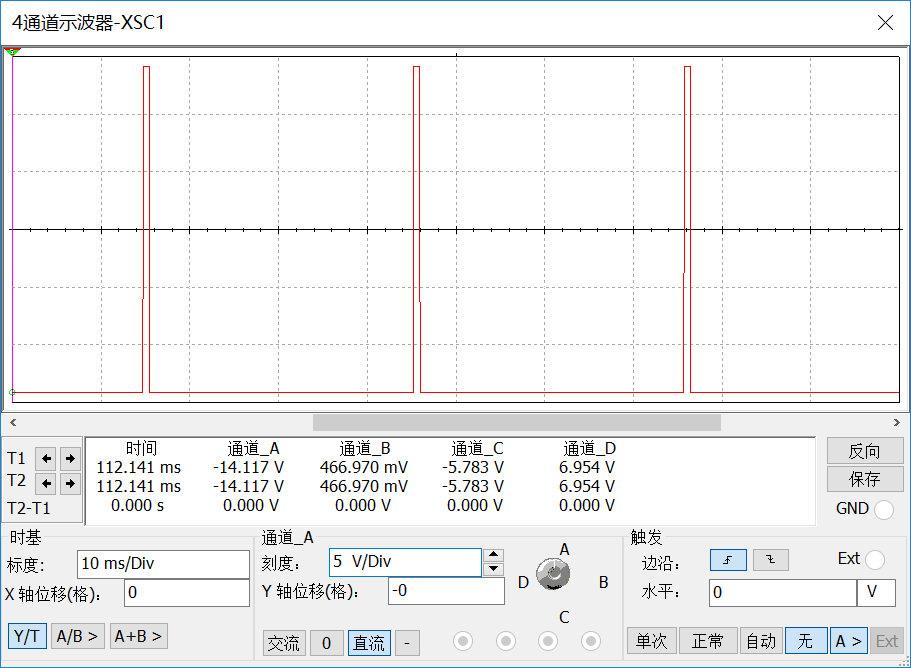
\includegraphics[width = 0.8\linewidth]{4/pulse.png}
	\caption{脉冲波形}
	\label{fig:脉冲波形}
\end{figure}

最终阶梯波形如图\ref{fig:向上阶梯波形}所示。符合设计要求,$ T = \SI{30}{\ms} $,输出电压幅值为\SI{10}{\V}左右。

\begin{figure}[H]
	\centering
	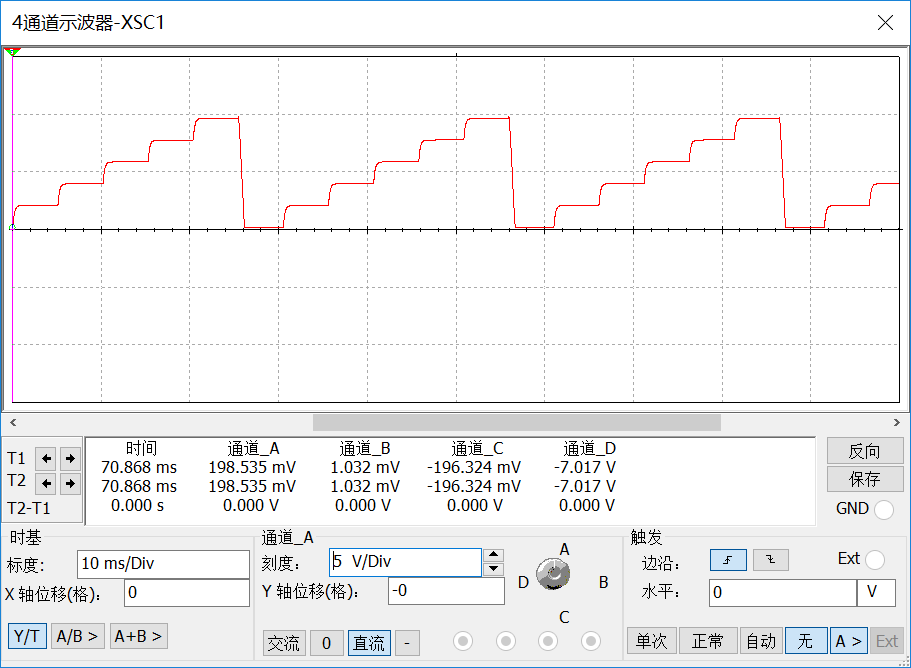
\includegraphics[width = 0.8\linewidth]{4/up.png}
	\caption{向上阶梯波形}
	\label{fig:向上阶梯波形}
\end{figure}

\subsubsection{向下阶梯波形}%
\label{ssub:向下阶梯波形}

如图\ref{fig:阶梯波发生器电路图},通过添加一个反相器可以得到向下阶梯波形。如图\ref{fig:向下阶梯波形}所示。

\begin{figure}[H]
	\centering
	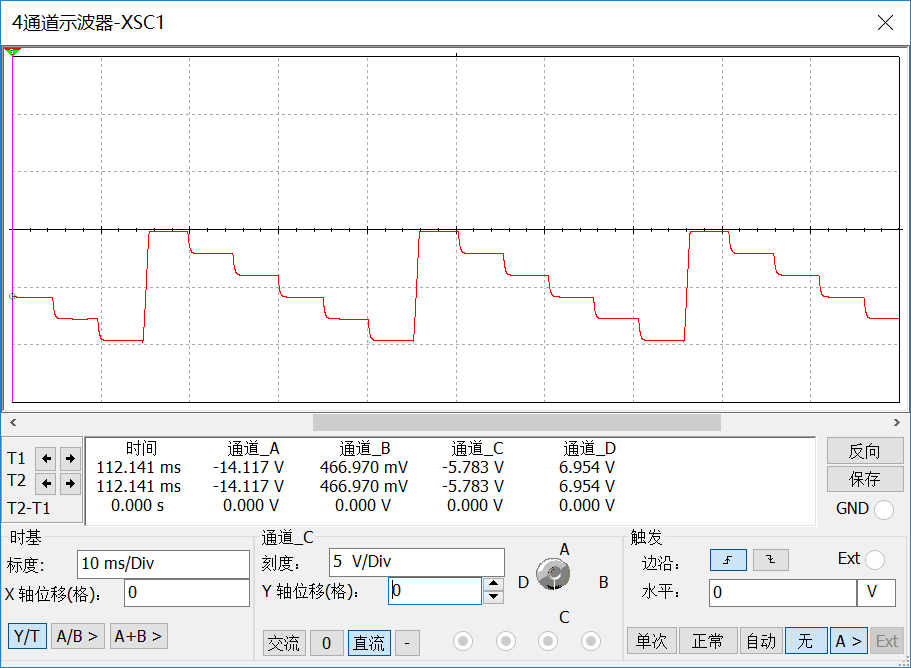
\includegraphics[width = 0.8\linewidth]{4/down.png}
	\caption{向下阶梯波形}
	\label{fig:向下阶梯波形}
\end{figure}

\subsubsection{三极管阶梯波发生器}%
\label{ssub:三极管阶梯波发生器}

\begin{figure}[H]
	\centering
	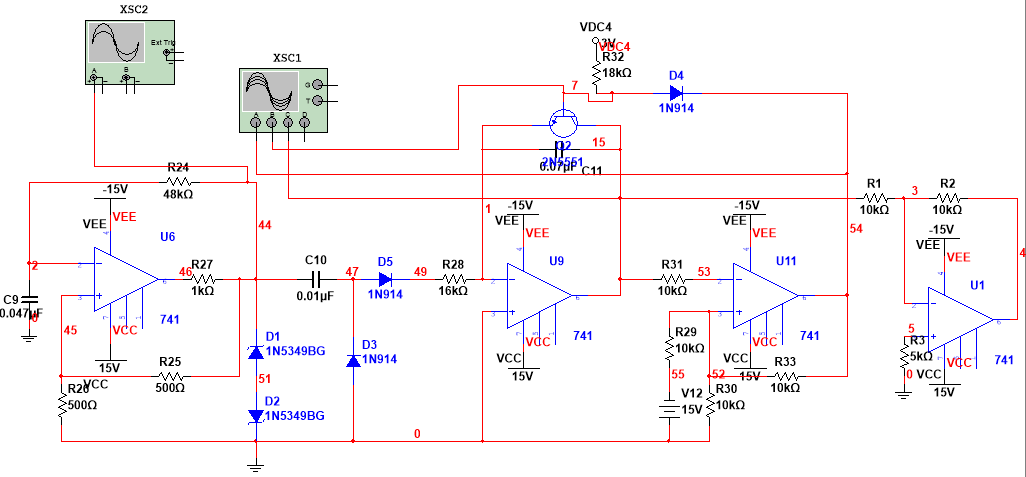
\includegraphics[width = \linewidth]{4/BJT.png}
	\caption{三极管阶梯波发生器}
	\label{fig:三极管阶梯波发生器}
\end{figure}

三极管阶梯波发生器电路图如图\ref{fig:三极管阶梯波发生器}所示。选用开关三极管替换
场效应管可以得到与原来阶梯波相近的波形。

\subsection{误差分析}%
\label{sub:\arabic{chapter}误差分析}

\begin{description}
	\item[阶梯波上升直线倾斜:]场效应管选择不当。
	\item[阶梯宽度不一致:]适当调节电阻大小,以重新满足周期要求。
	\item[毛刺:]门限电平未能控制好,调节电阻使门限电平尽可能接近\SI{10}{\V}。
\end{description}

\section{实验小结}%
\label{sec:\arabic{chapter}实验小结}

在这次实验中设计了一个具有一定功能的电路。先将一个项目细分为小的问题,再逐一解决。在这期间,查资料、计算、对相应的电路进行测验以检测其正确性。

这是通过Multisim进行设计仿真,对搭建实际电路有巨大的帮助作用。通过仿真软件,设计人员可以轻松的进行电路设计、参数调整。这对解决实际问题有着巨大的帮助。


\chapter{结论}%
\label{cha:结论}

本次实验运用Multisim软件进行仿真实验,完成相应问题,经历了电路设计的流程,对实验结果进行与理论值进行分析比较。巩固了模拟电子线路的一些知识,对于三极管、场效应管、运算放大器等元件有了较深的理解。设计电路时,涉及到模拟电路知识,需要复习相关知识点;在运用中,加深理解。调整电路时,根据公式调整元件参数,会使调整快捷、准确,节省大量时间,提高工作效率。

这一阶段,学习了一些仿真软件的分析方法,这为分析电路的性能,提供了强大的工具,方便设计者设计分析。

在以后的学习中,遇到相关问题,也可以运用这种工具加以分析。



% Fakesection 参考文献

\addcontentsline{toc}{section}{参考文献}

\bibliographystyle{IEEEtran}
\bibliography{bib/main}

\end{document}

